\documentclass{beamer}
\usepackage{amsfonts, amsmath, graphicx, verbatim, graphicx, hyperref,
  color}
\definecolor{UNBlue}{RGB}{91, 146, 229}
\setbeamercolor{structure}{fg=UNBlue}
\newcommand\Fontvi{\fontsize{6.5}{7.2}\selectfont}
\usetheme{Warsaw}

\title{Imputation of the Production Domain}
\author{\it Michael C. J. Kao}
\institute{Food and Agriculture Organization \\ of the United Nations}
\date{}

\AtBeginSection[]
{
  \begin{frame}<beamer>
    \frametitle{Outline for section \thesection}
    \tableofcontents[currentsection]
  \end{frame}
}

\begin{document}

\frame{
  \titlepage
  \centering
  
\includegraphics[scale = 0.2]{fao_logo.png}
}

\frame{
  \frametitle{Outline}
  \tableofcontents
}


\section{Introduction}
% \frame{
%   \frametitle{Introduction}

%   The agricultural production domain is integral to the compilation of
%   Food Balance Sheets. In particular to estimate consistent food
%   supplies, imputation is required to ensure that data are non-sparse.

%   \vfill

%   Owing to the potential impact of imputation when often data are
%   missing, accuracy and reliability of food estimates cannot be
%   compromised.

% }


\frame{
  \frametitle{Relationships}

  The relationship of production and its components by definition can
  be expressed as:

  \begin{equation}
    \label{eq:pae}
    P_t := A_t \times Y_t \, \, \, \,\,\,\, P_t \ge 0, A_t \ge 0, Y_t > 0
  \end{equation}

  \vfill
  Where $P_t$ , $A_t$ and $Y_t$ denotes production, area harvested
  and yield, respectively, at time t.

}

% \frame{
%   \frametitle{Relationships}
%   Sometimes it may be more convinient to express the relationship in
%   the logarithmic scale. Where the relationship becomes an additive
%   one.

%   \begin{equation}
%     \label{eq:lpae}
%     \log(P_t) := \log(A_t) + \log(Y_t) \, \, \, \,\,\,\, P_t > 0, A_t >
%     0, Y_t > 0
%   \end{equation}

%   \vfill
%   When production and area harvested are both missing or zero, the
%   yield is missing and needs to be imputed.

% }


\frame{
  \frametitle{Scope of the project}

  A total of \textbf{169} commodity just in the crop domain.

  \vfill

  \textbf{228} countries including obsolete classification and
  territories.

  \vfill

  A total of \textbf{31,797} time series require imputation.

  \vfill

  Percentage of missing value can be as high as \textbf{80\%} (By
  commodity).

}


% \frame{
%   \frametitle{Outline}

%   In this seminar, we will illustrate the proposing methodology for
%   imputation of the production domain starting from yield, then
%   production and area harvested.

%   \vfill

%   % Finally a balancing step to ensure the equation are satisfied and
%   % statistically valid.

% }


% \section{Imputation}
\section{Yield}
\frame{
  \frametitle{Linear mixed model}

  The model implemented in for the imputation of yield is the linear
  mixed model.

  \vfill

  It is an extension of the simple linear regression, but enables the
  user to take advantage of any correlation structure exist.

}

\frame{
  \frametitle{Yield of grape}
  % Start by looking at the country level
  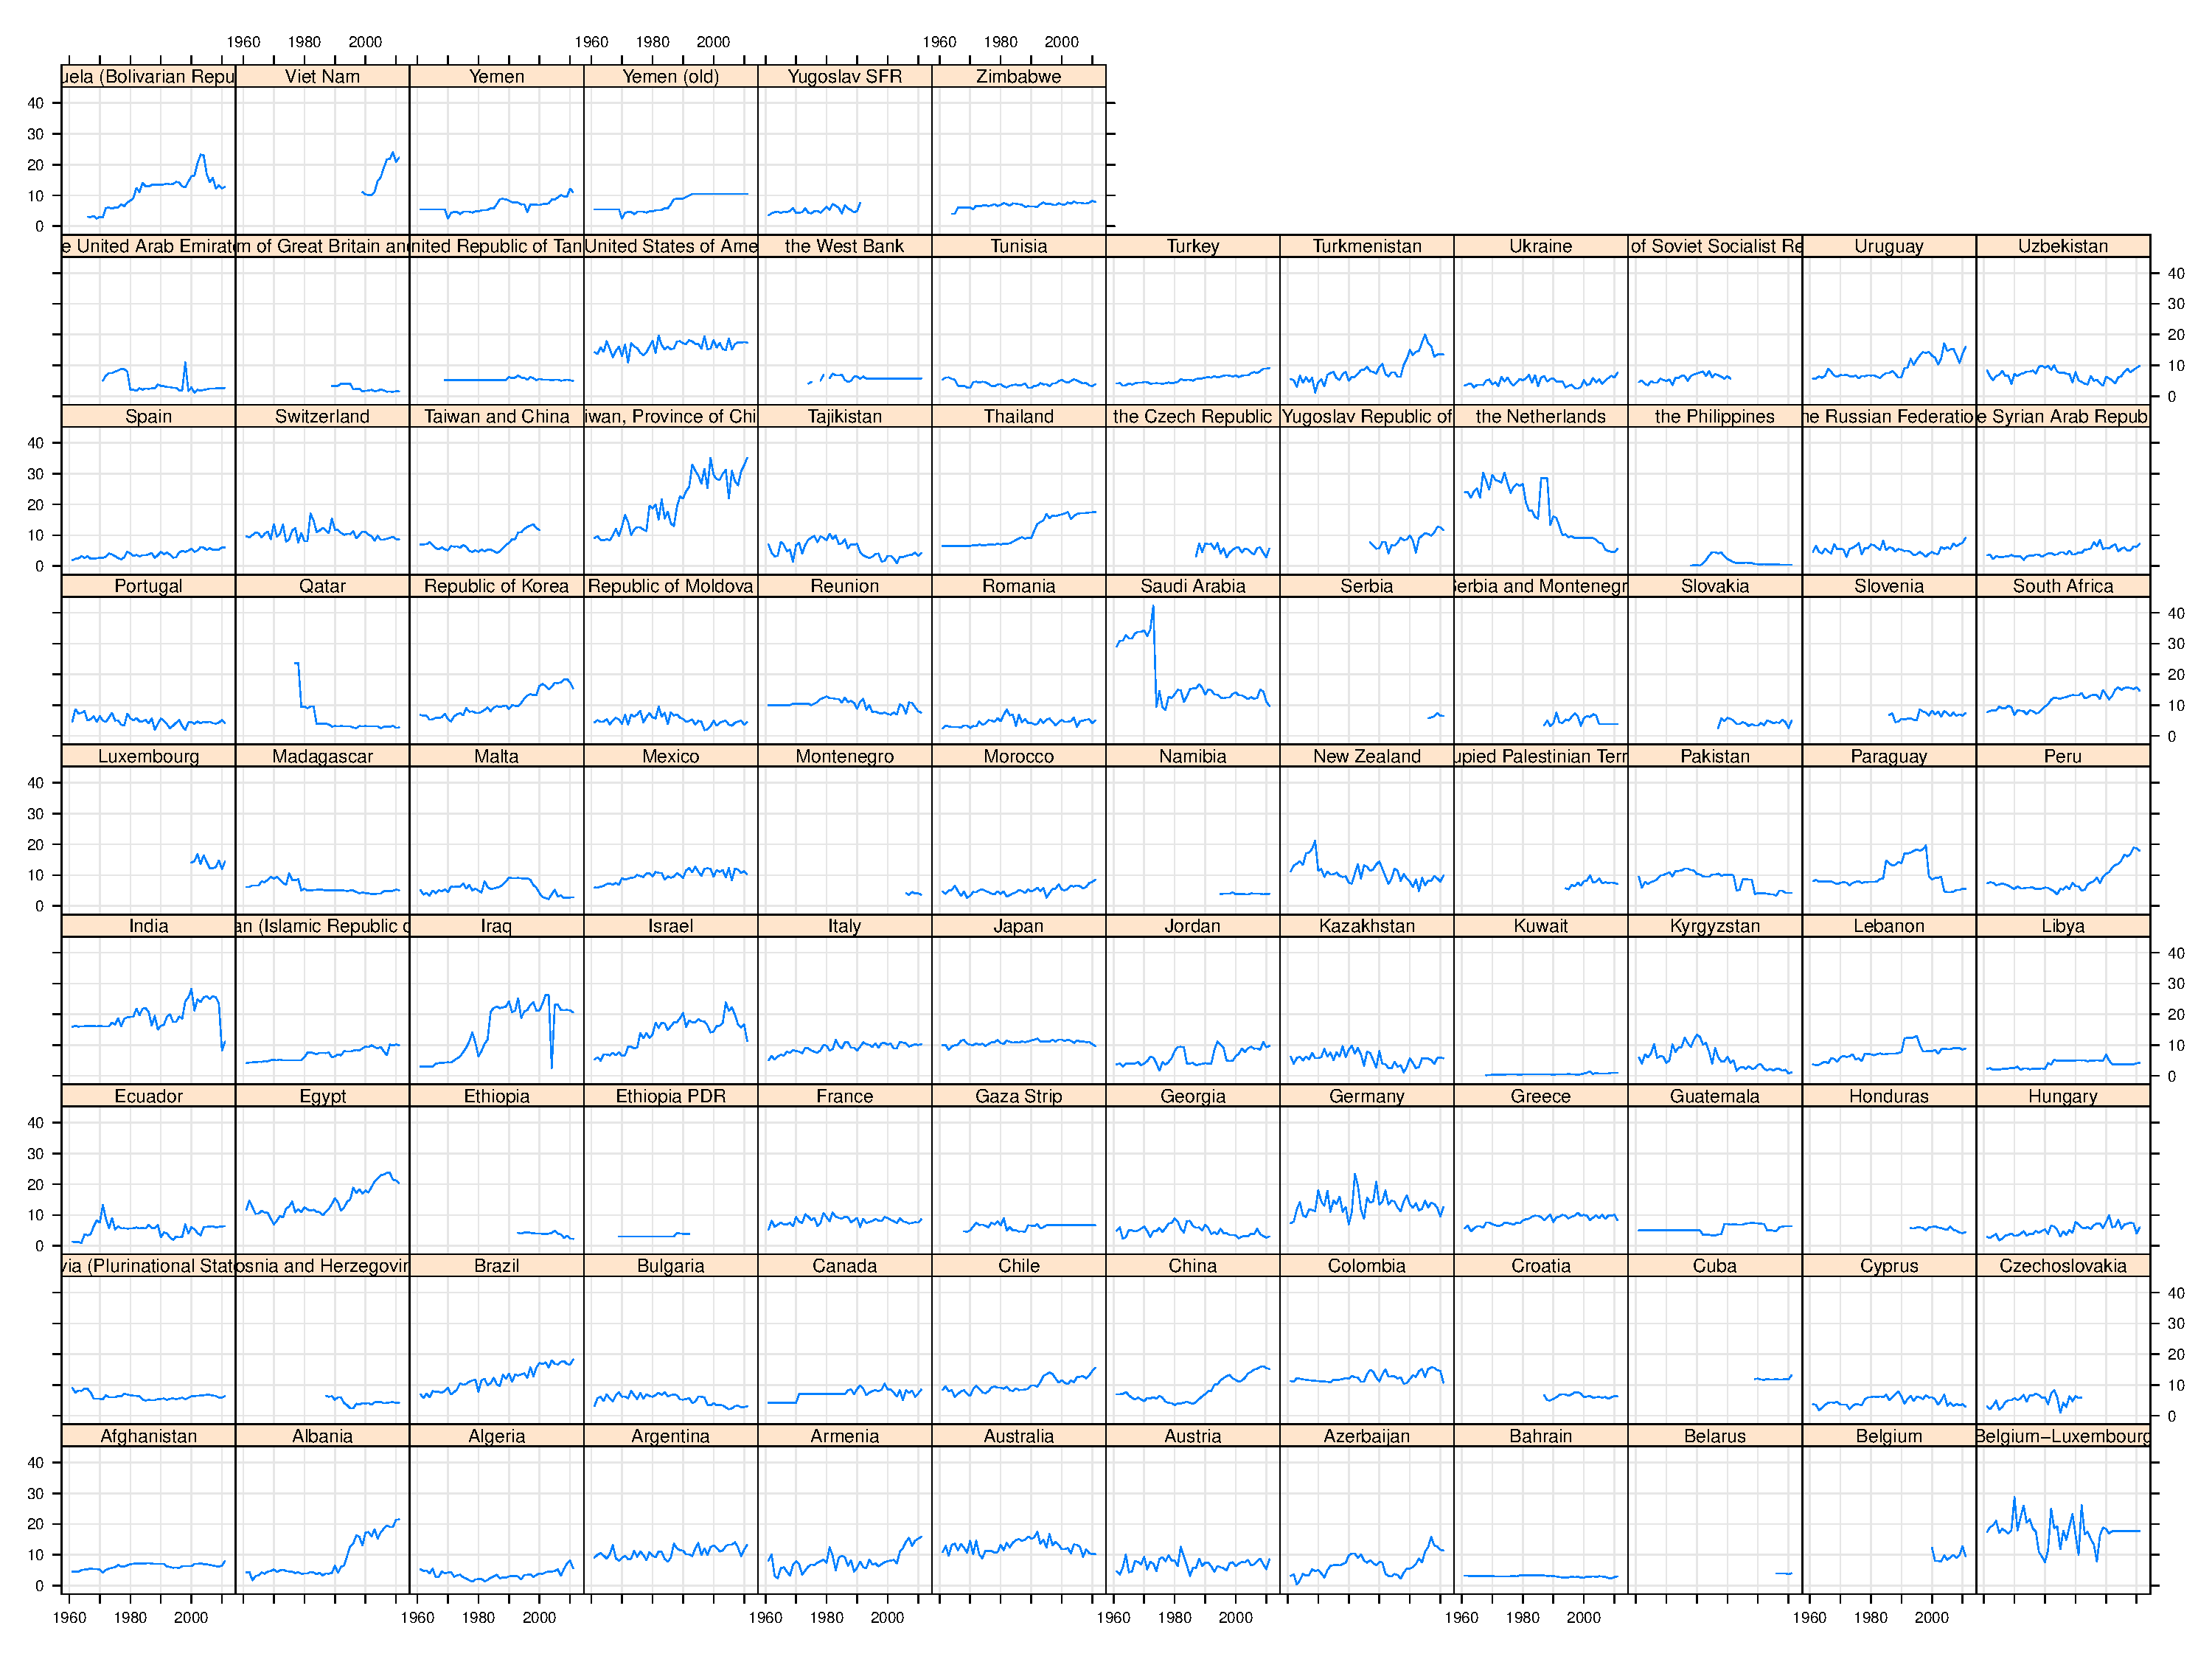
\includegraphics[scale = 0.2]{grapeYieldRaw}
}

\frame{
  \frametitle{Global Model}
  % illustrate a global fit where it can not adequately capture the
  % pattern.
  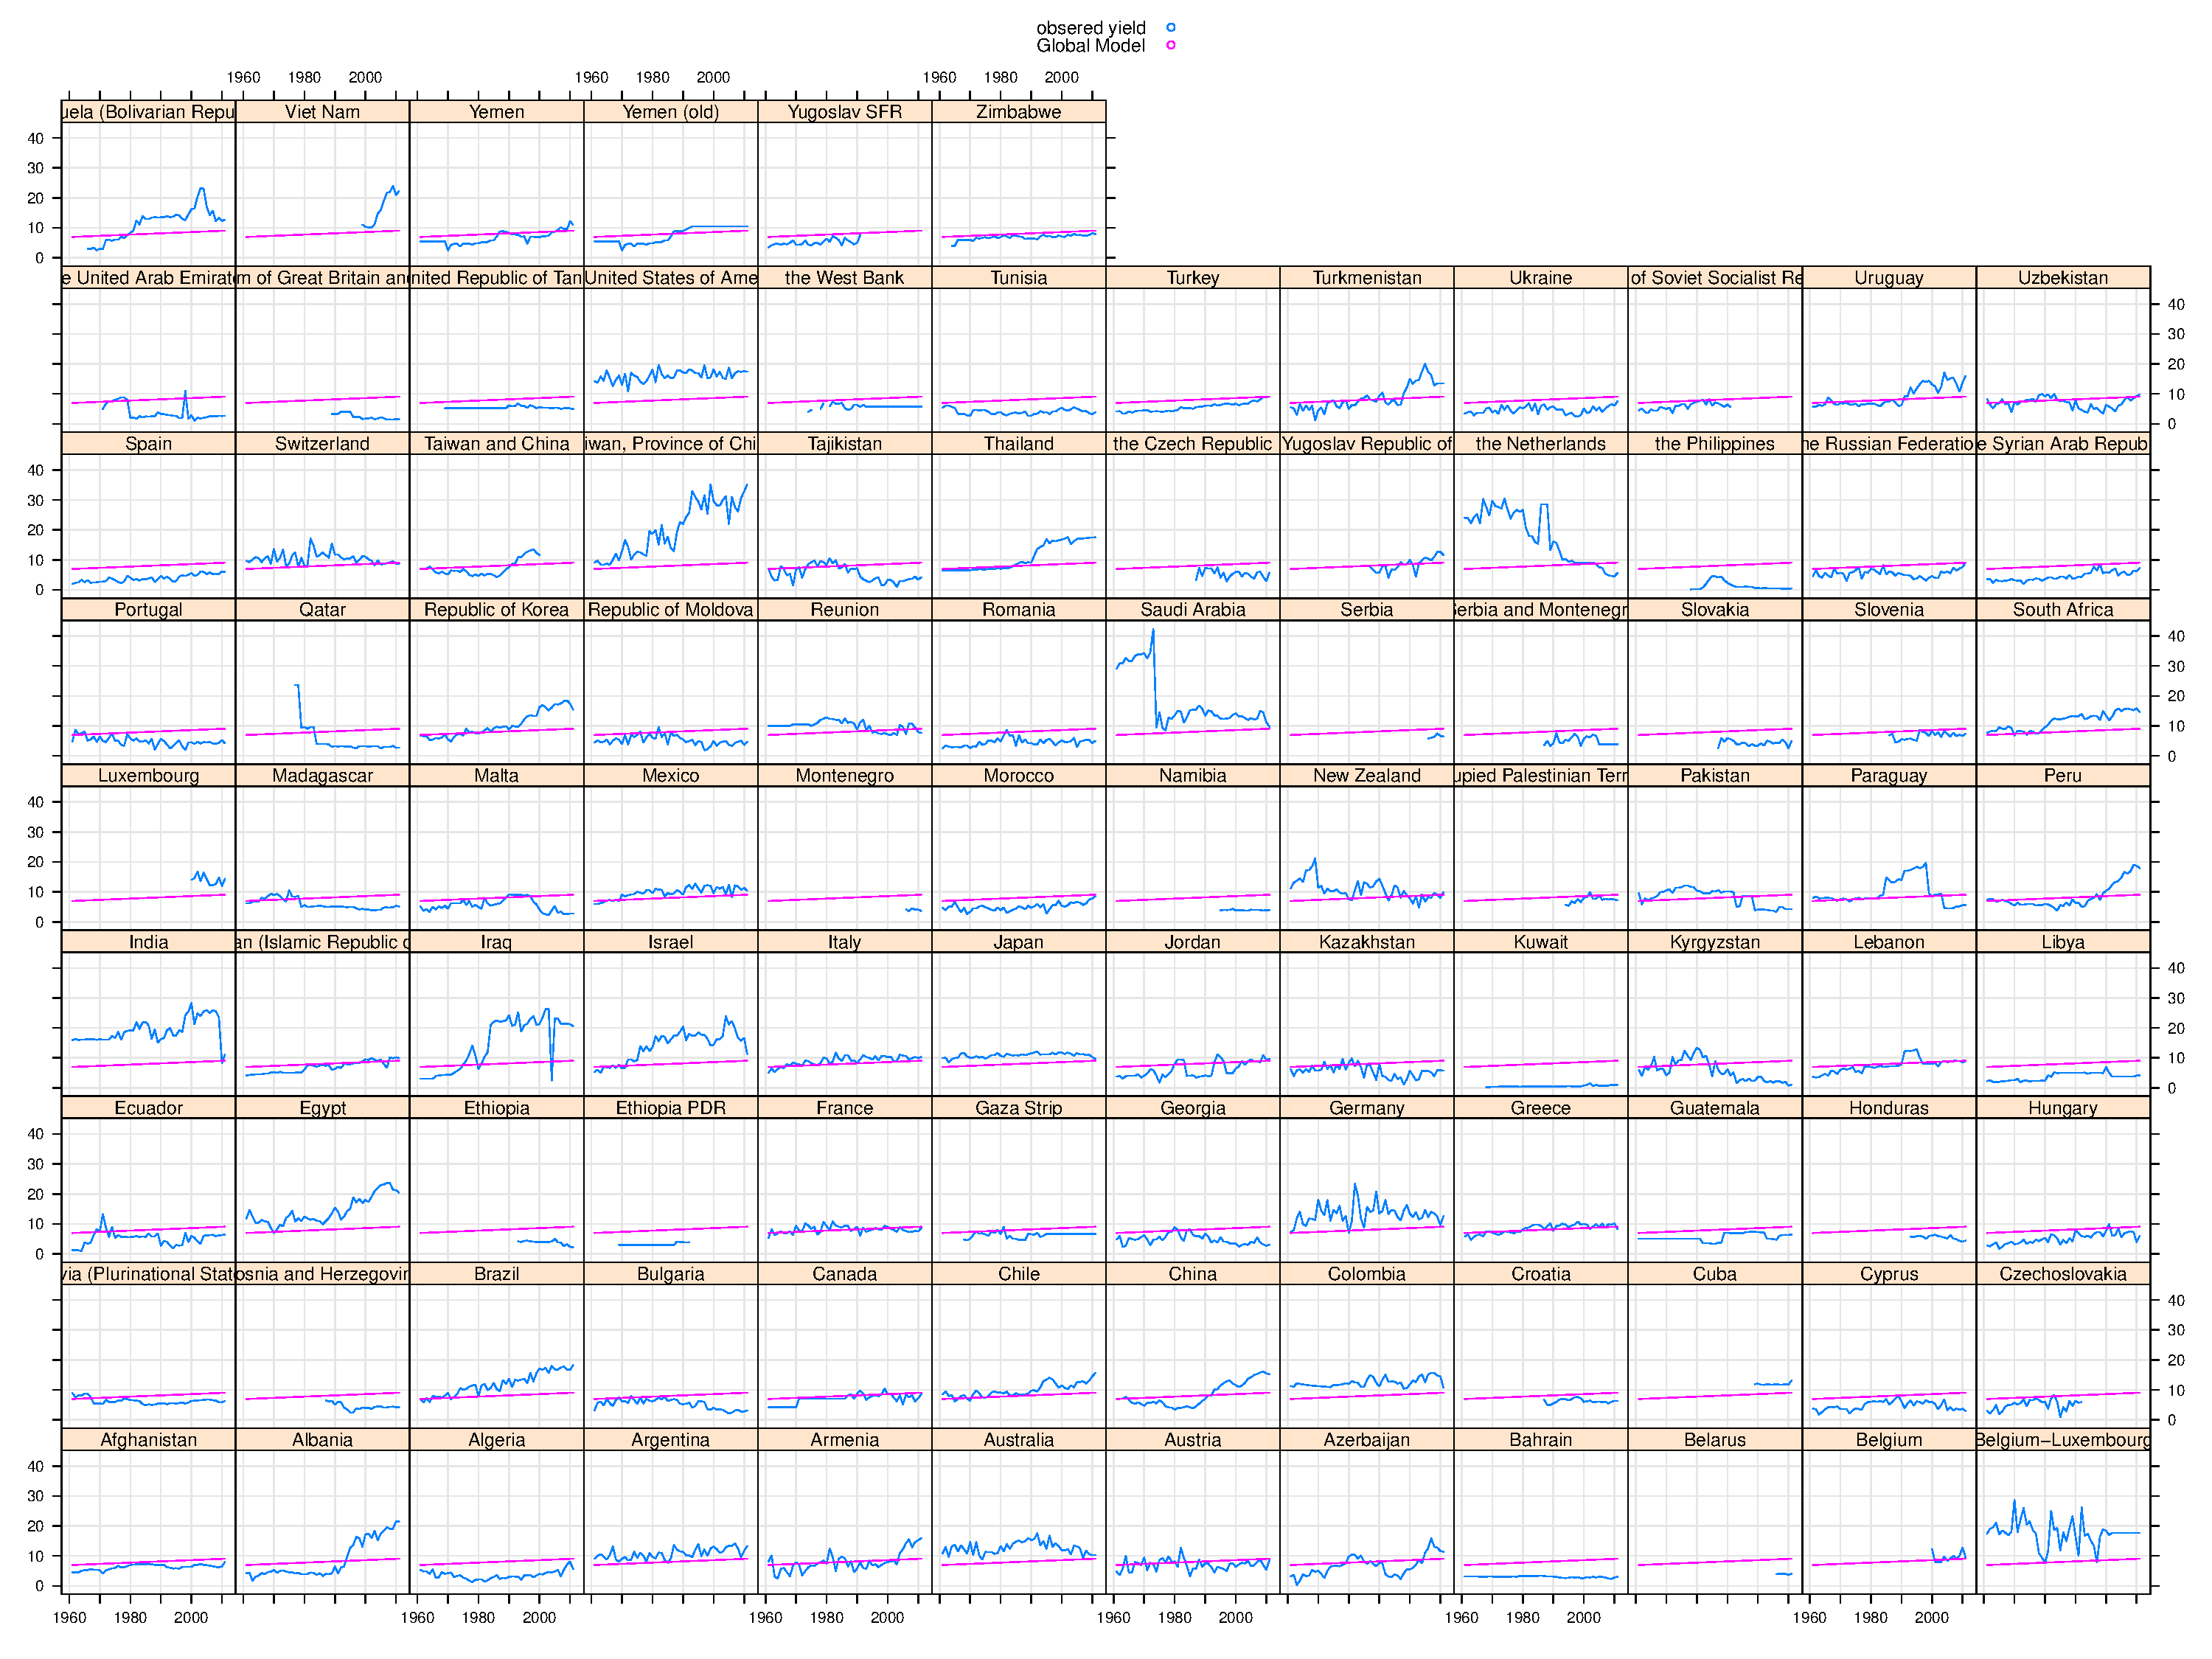
\includegraphics[scale = 0.2]{grapeYieldGlobal}
}

\frame{
  \frametitle{Country Model}
  % illustrate a country-by-country fit and show how it can fail when
  % the number of points are small and the slope can be very volatile.
  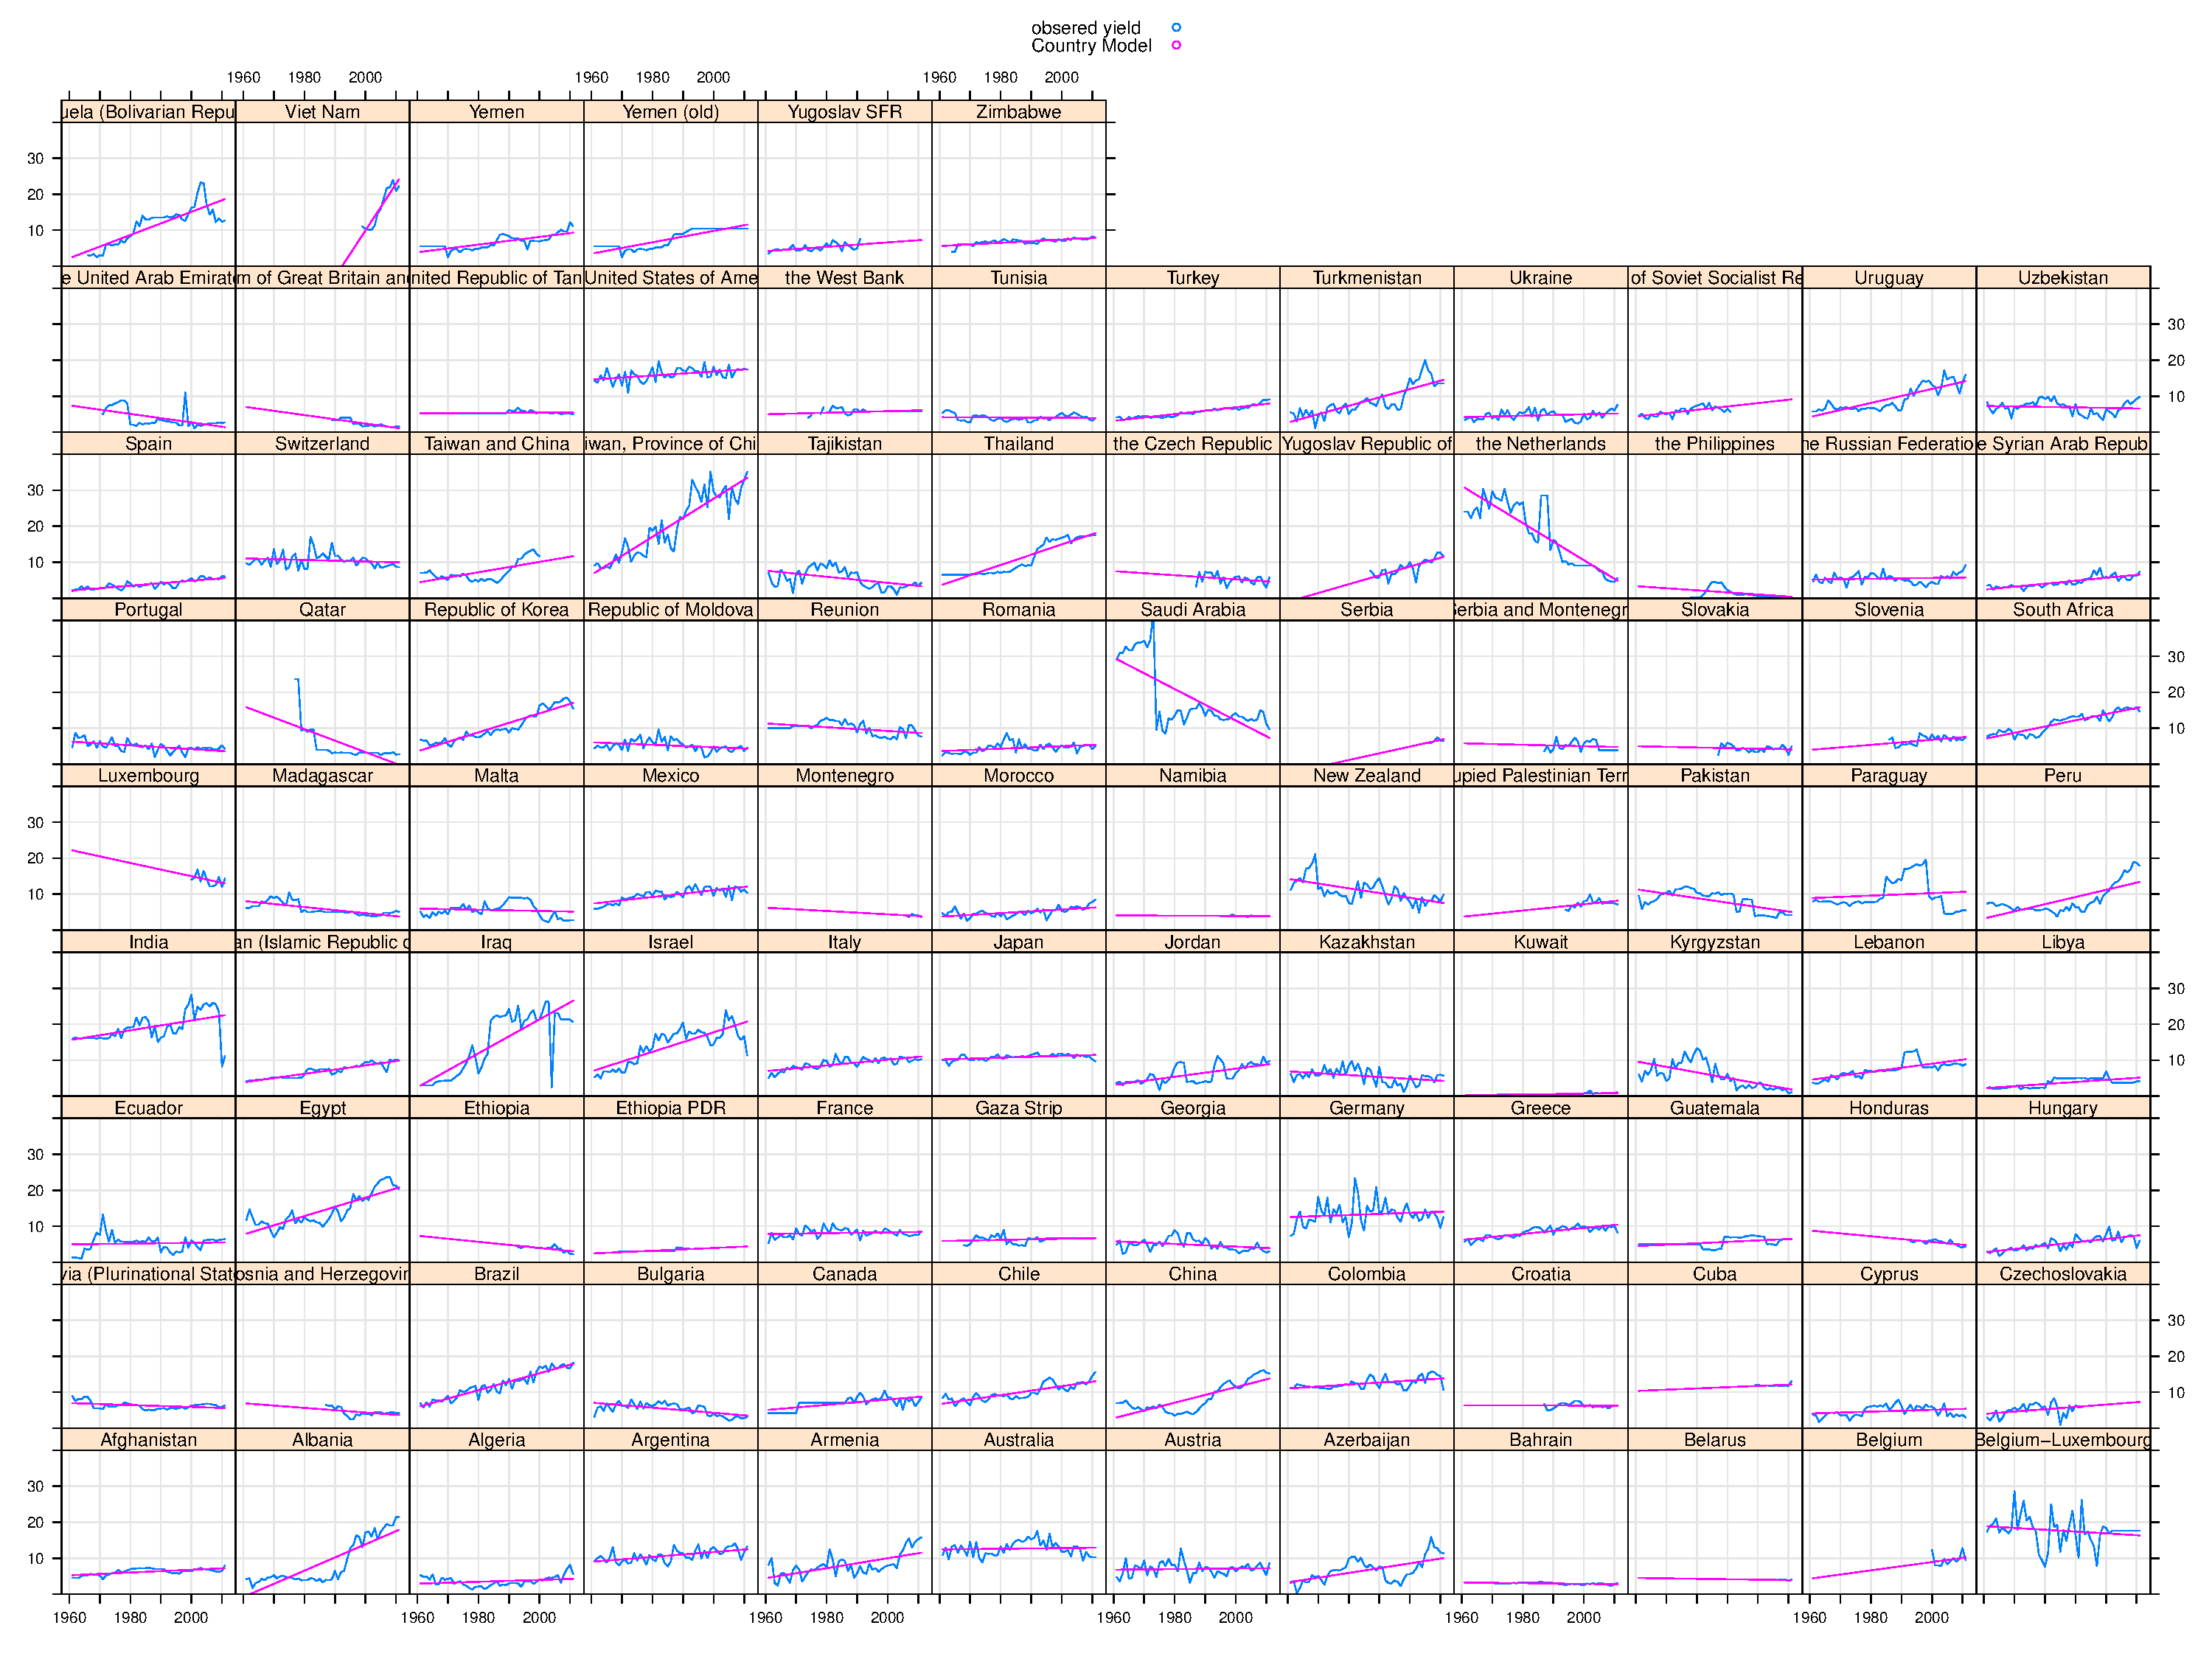
\includegraphics[scale = 0.2]{grapeYieldCountry}
}

\frame{
  \frametitle{Linear Mixed Model}
  % Illustrate how the linear mixed model solve the problem shown in
  % the previous two slide.
  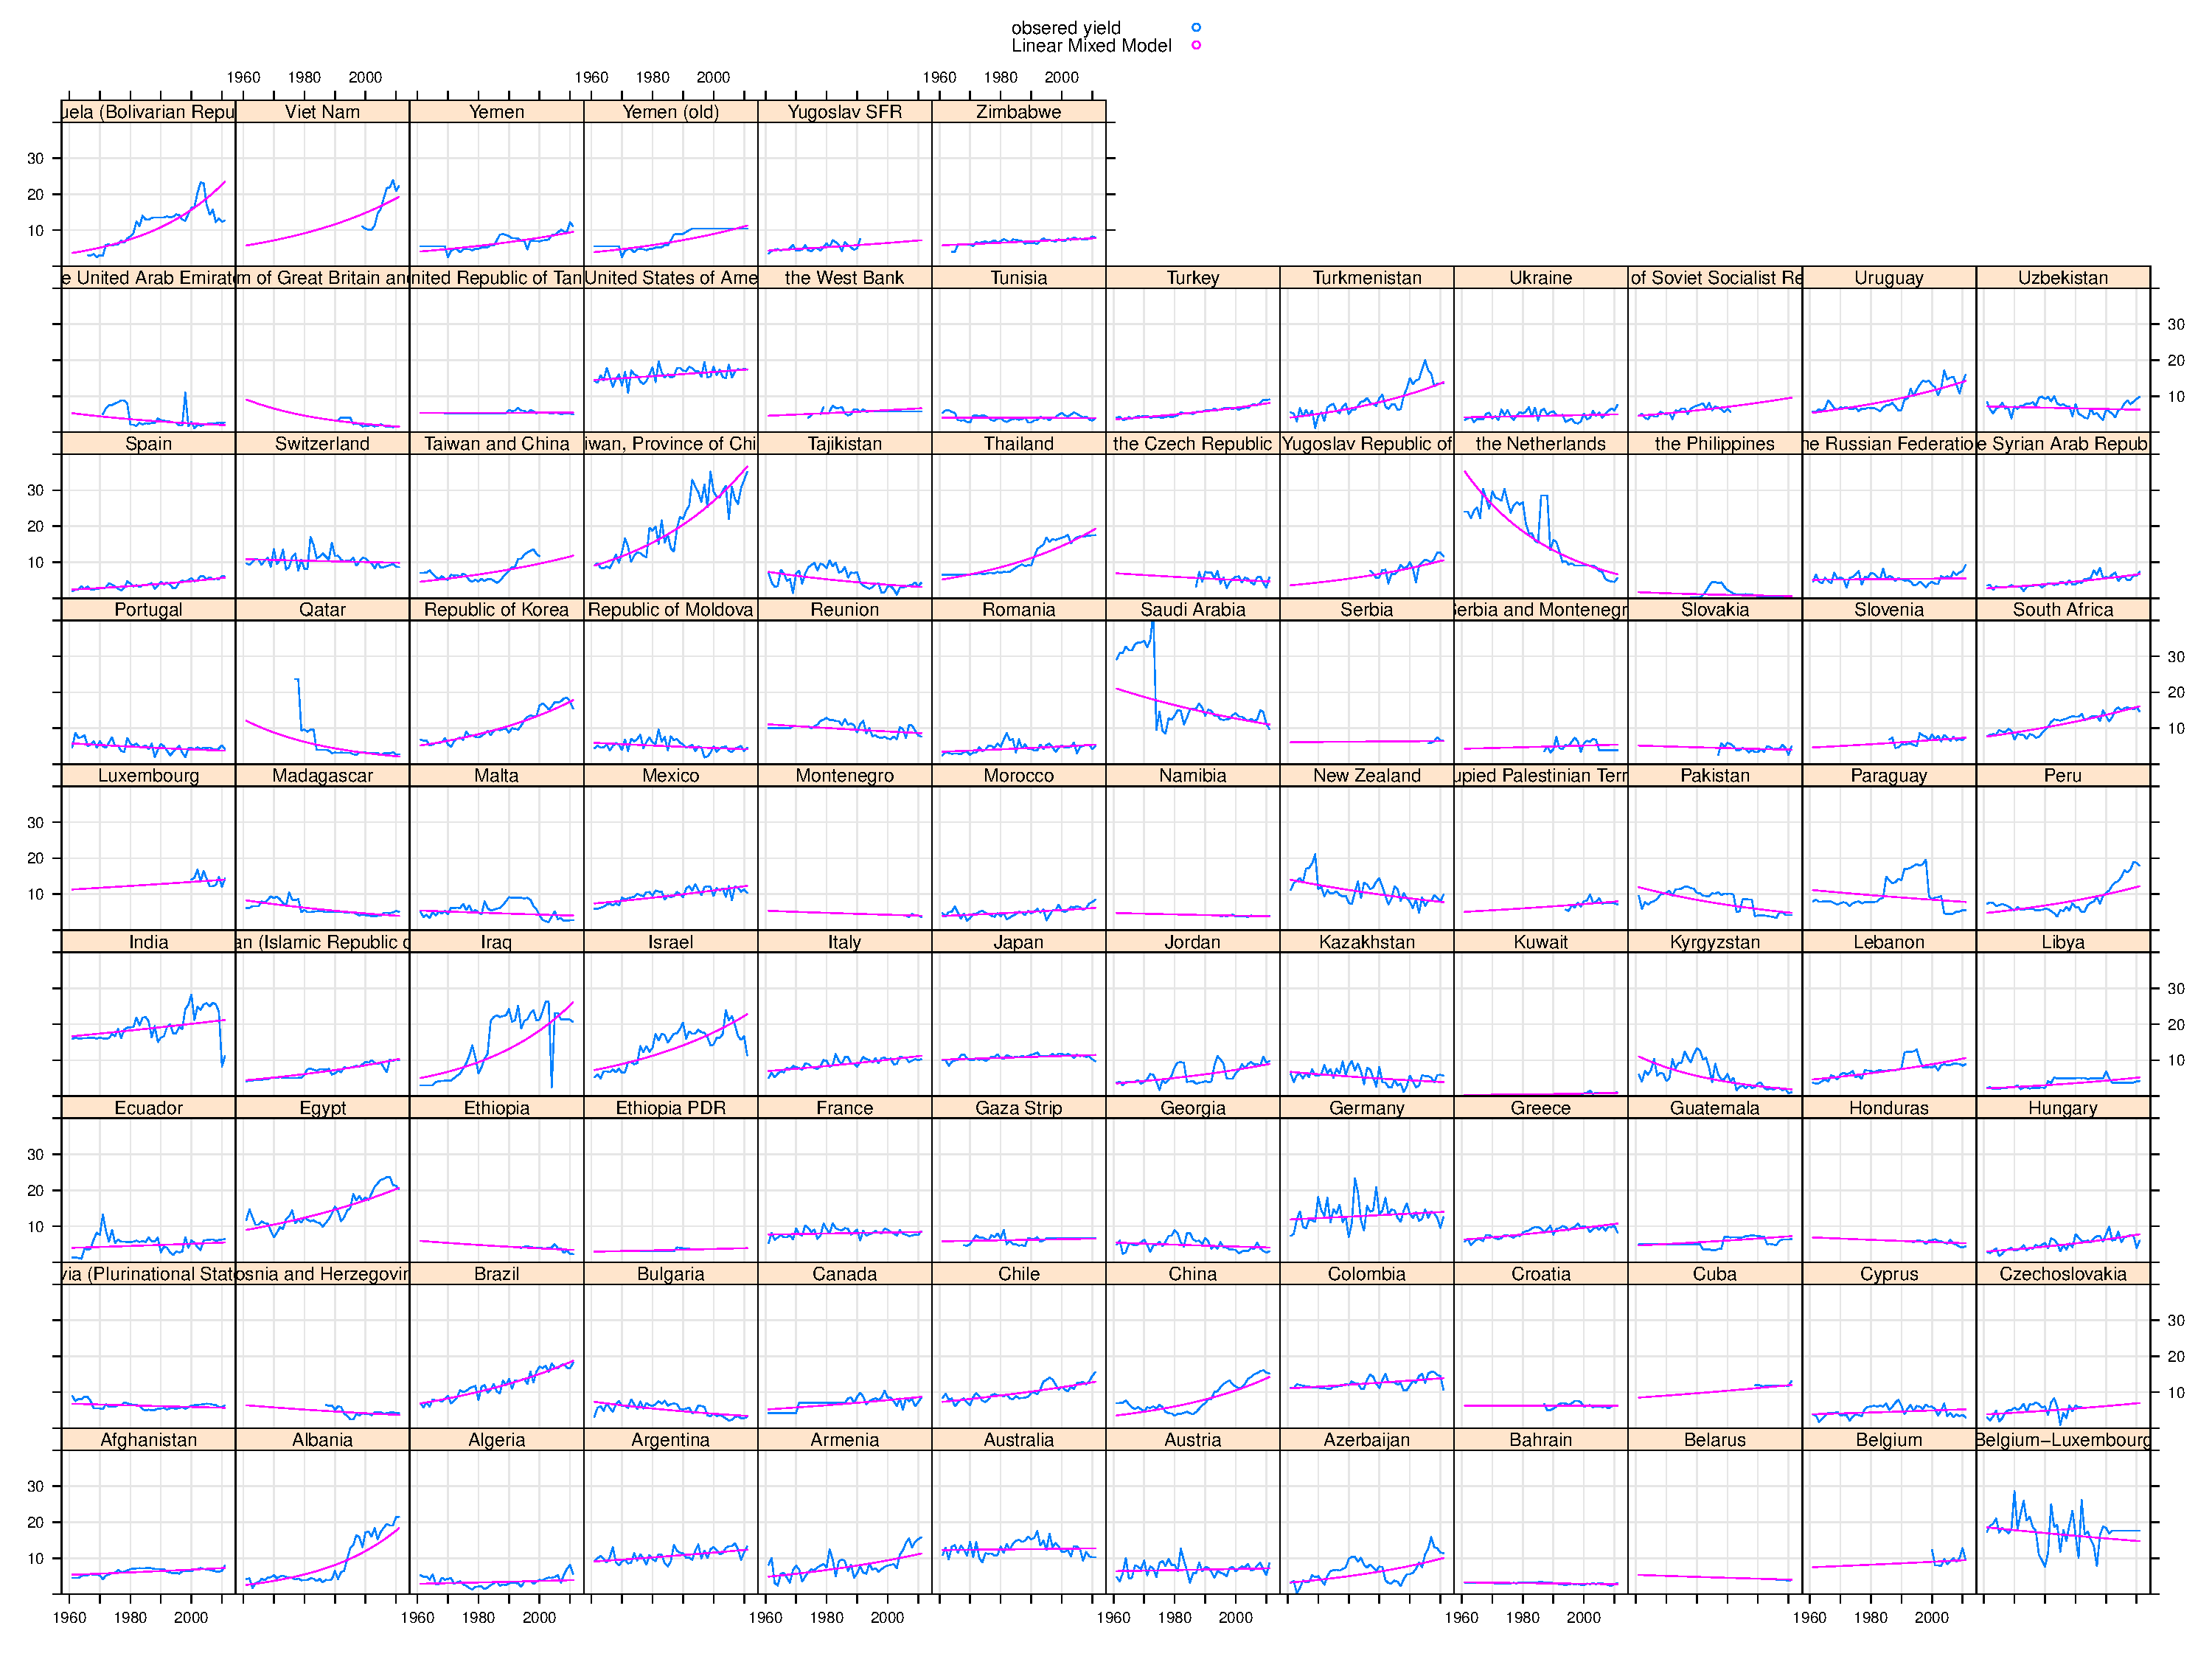
\includegraphics[scale = 0.2]{grapeYieldLme}
}

\frame{
  \frametitle{Linear Mixed Model with Splines}
  % Illustrate how the linear mixed model solve the problem shown in
  % the previous two slide.
  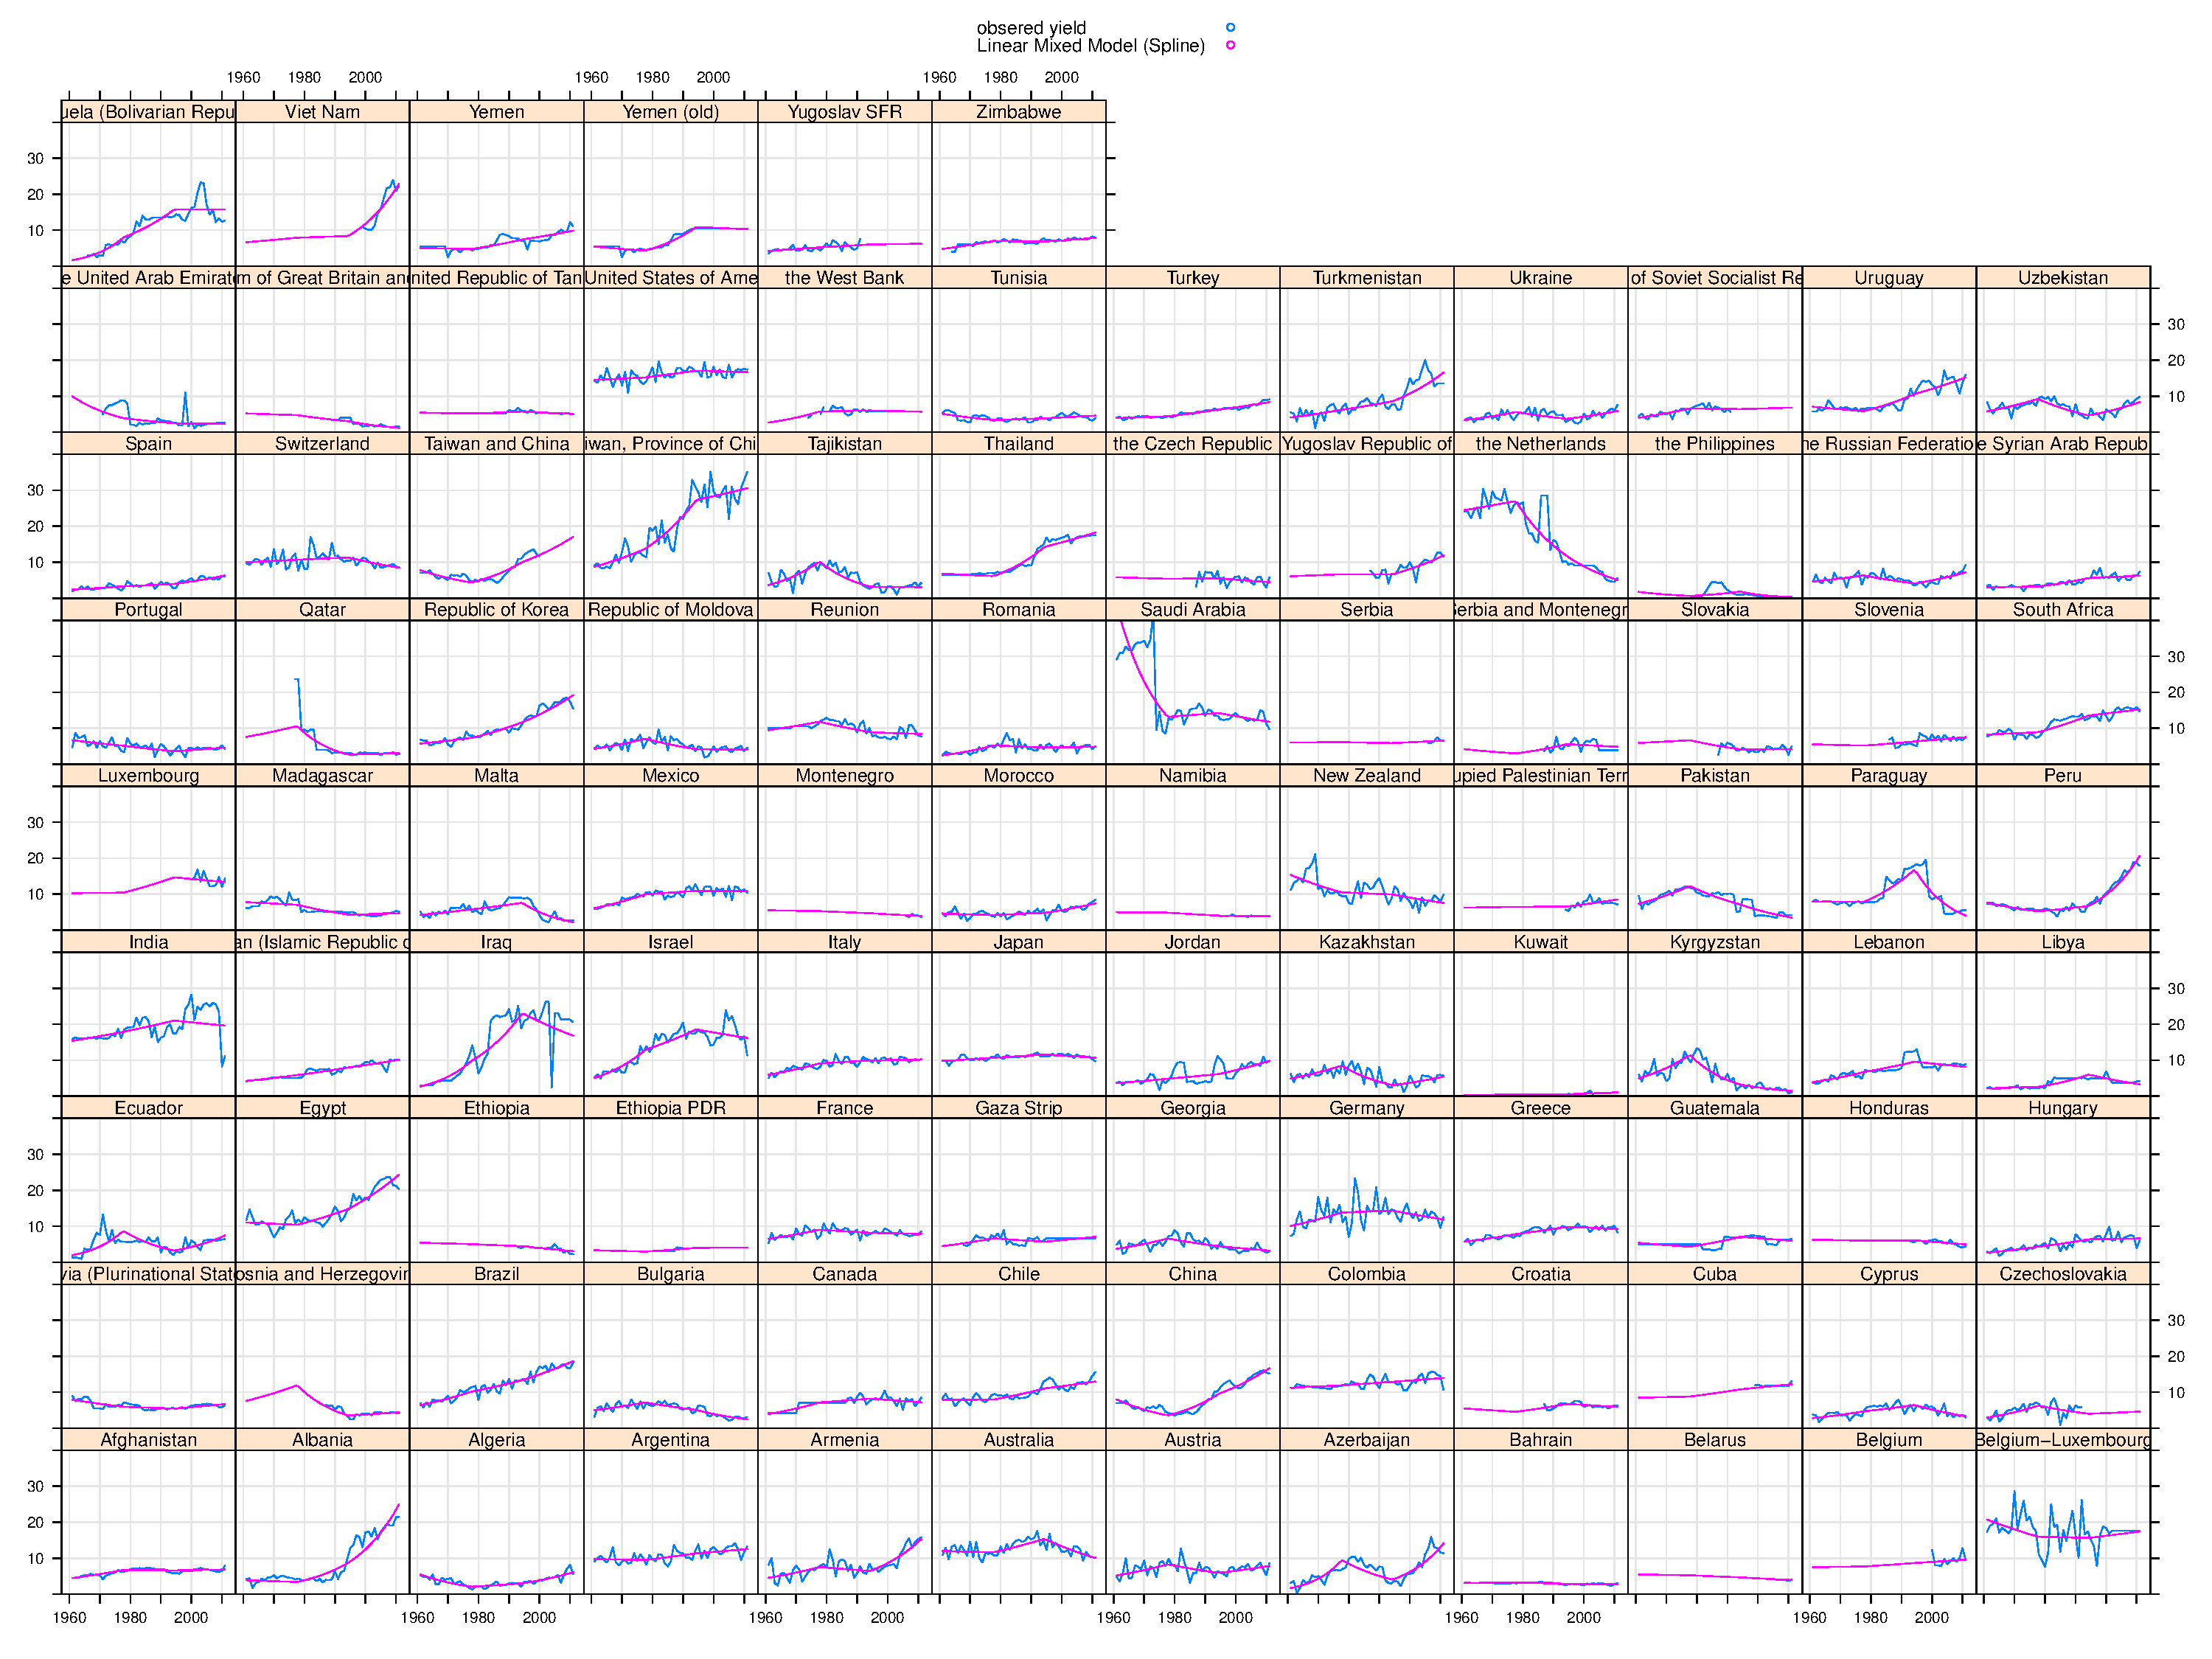
\includegraphics[scale = 0.2]{grapeYieldSplineLme}
}

\frame{
  \frametitle{Yield of green peas}
  % Start by looking at the country level
  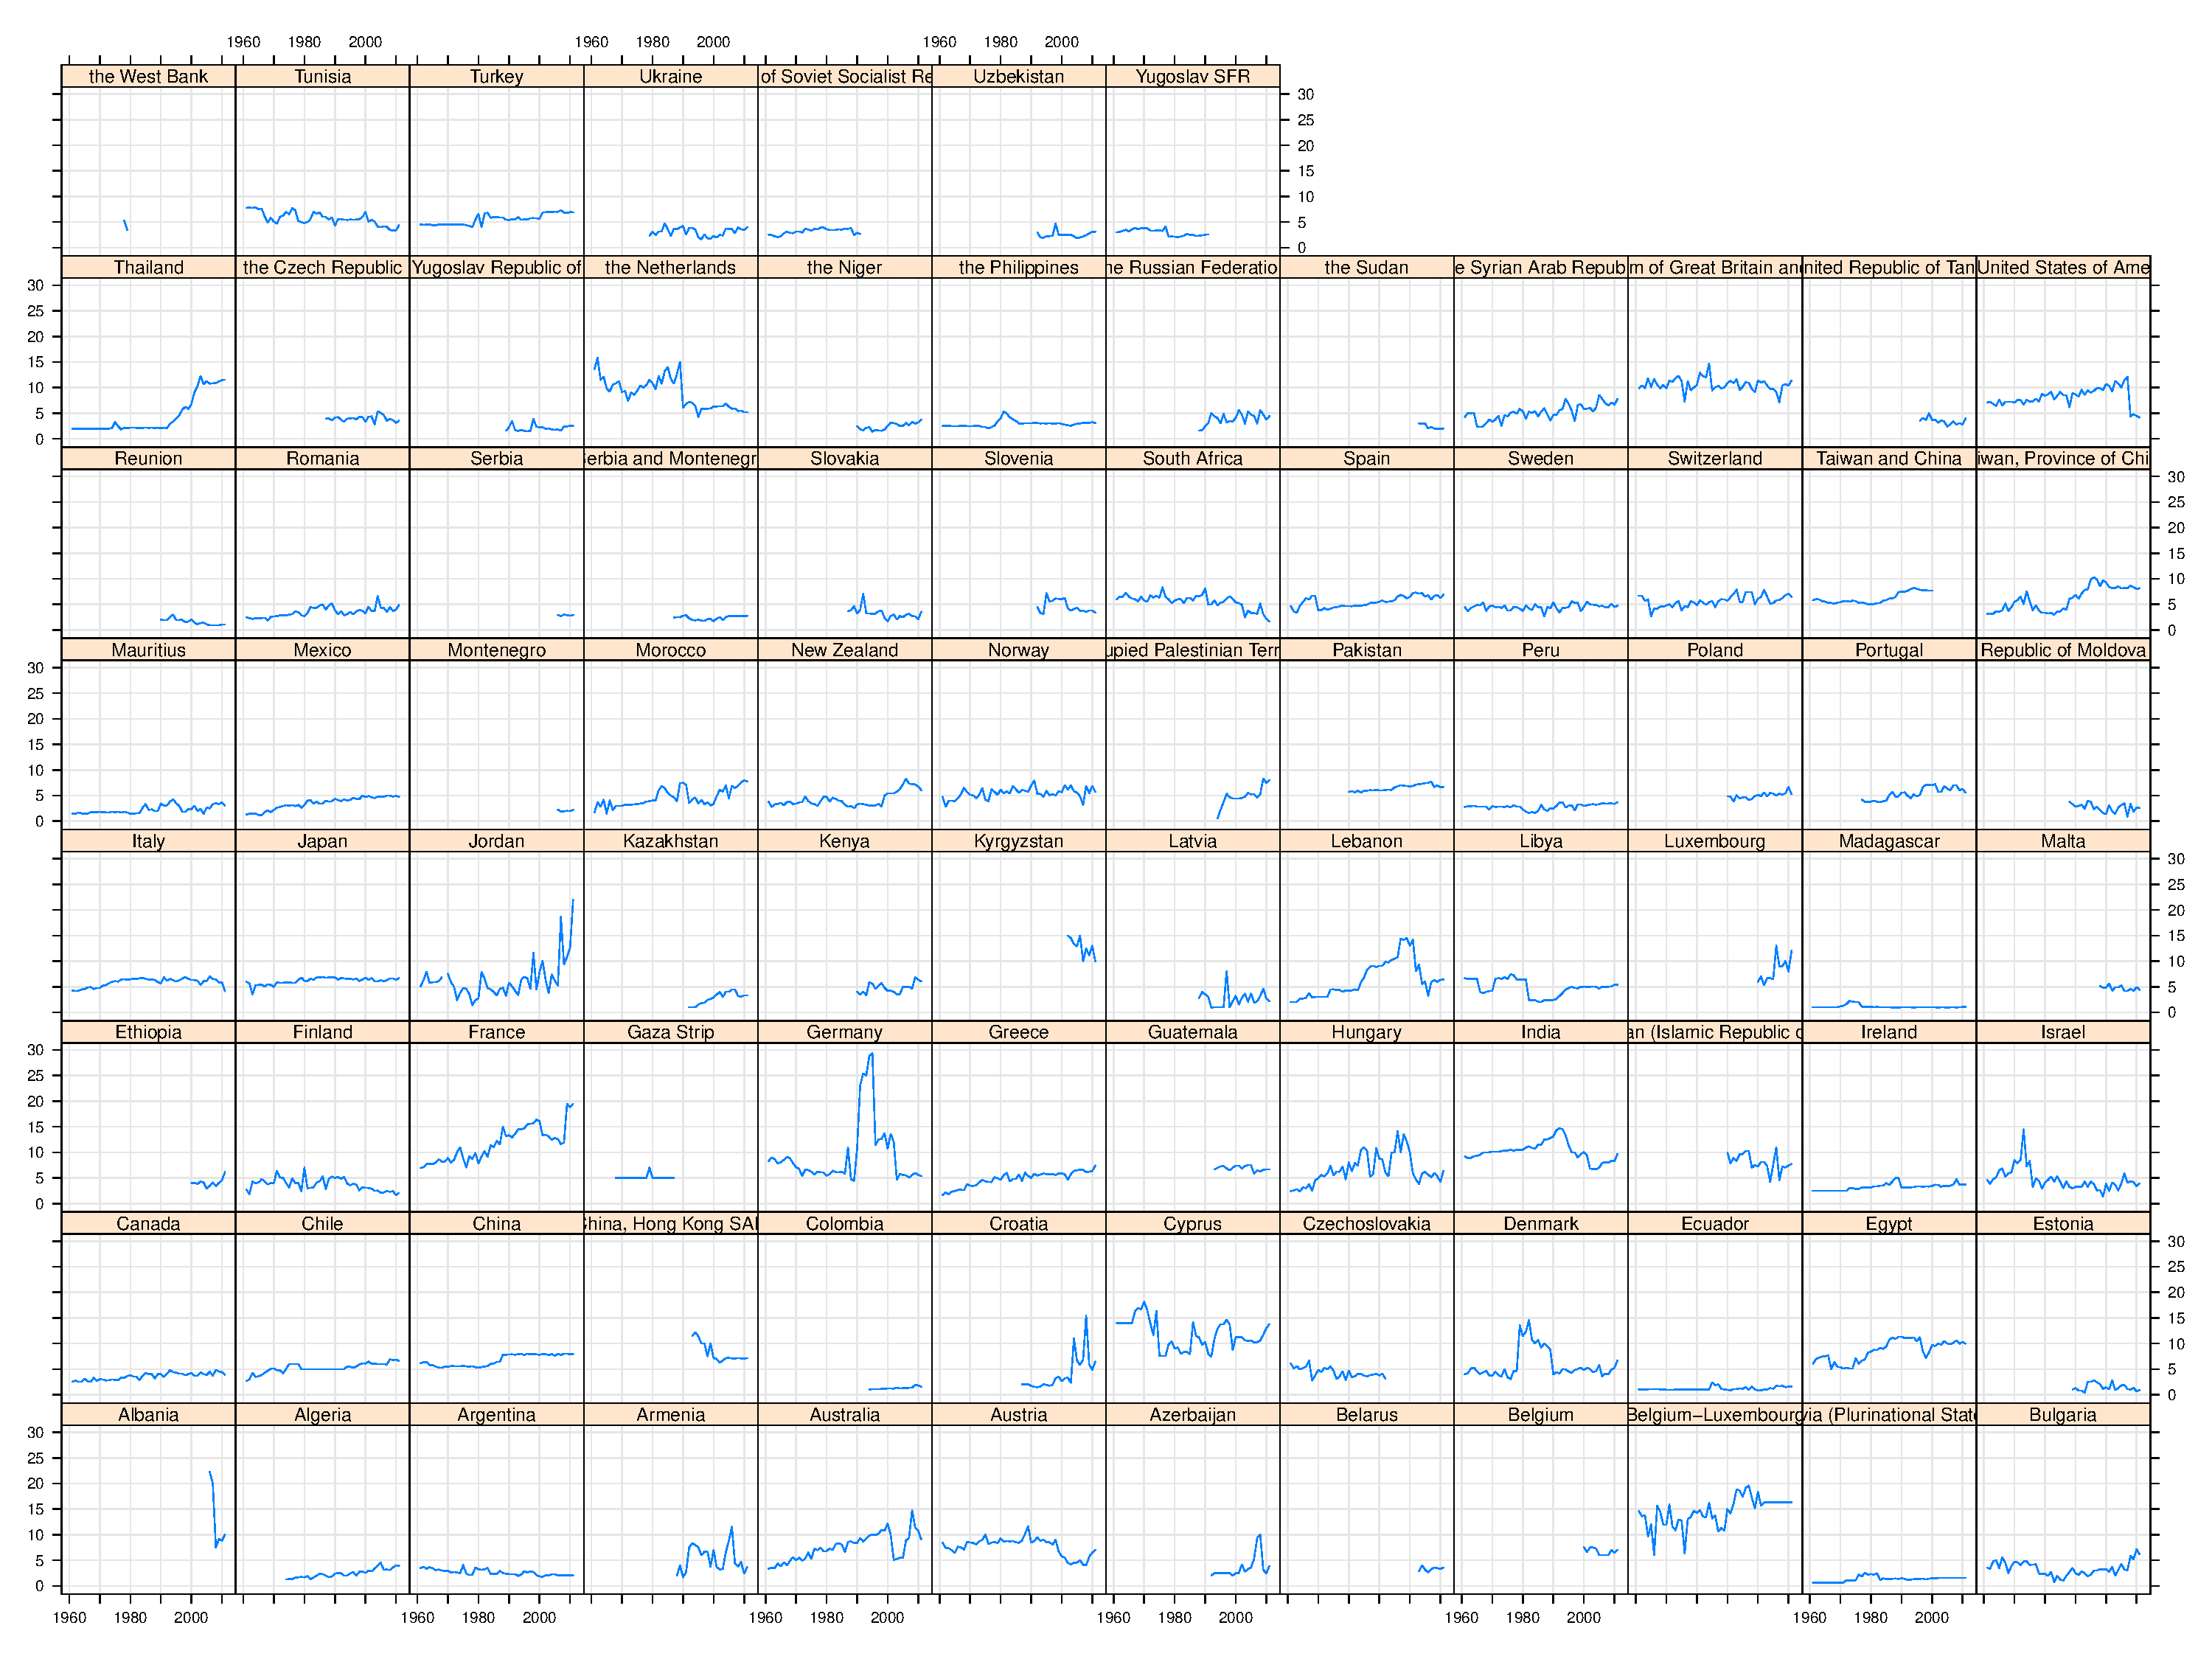
\includegraphics[scale = 0.2]{peasGreenYieldRaw}
}

\frame{
  \frametitle{Global Model}
  % illustrate a global fit where it can not adequately capture the
  % pattern.
  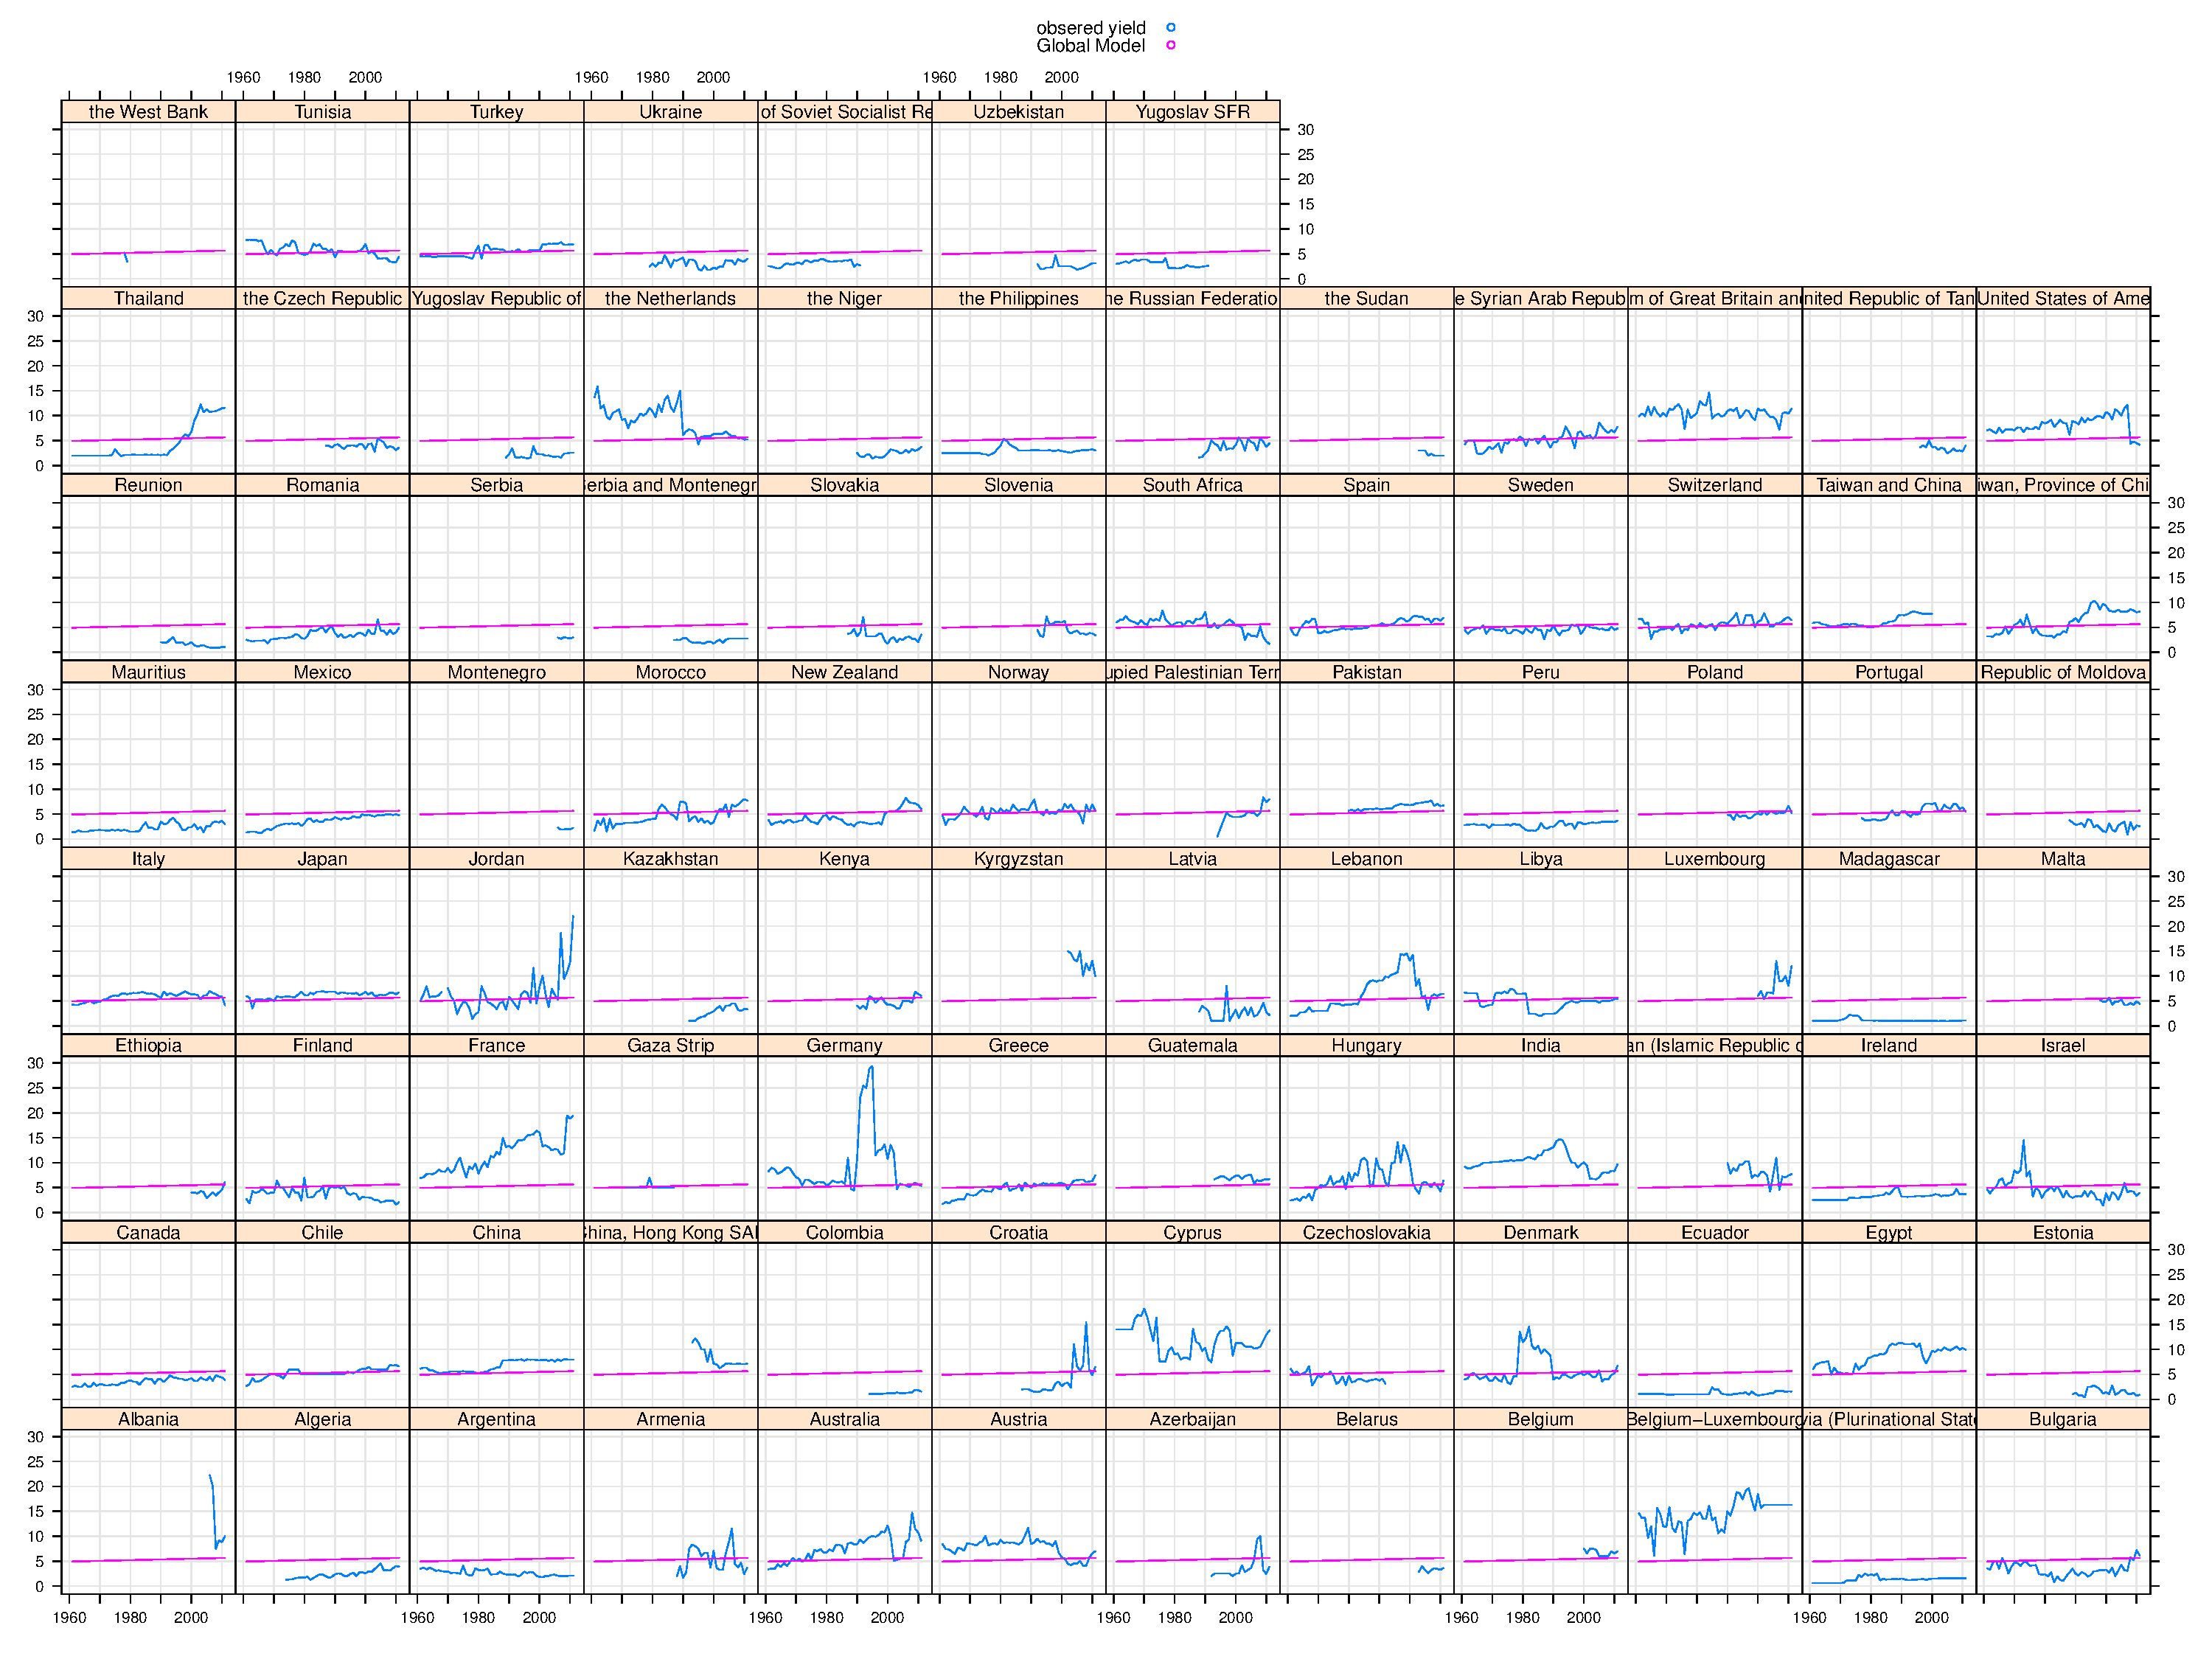
\includegraphics[scale = 0.2]{peasGreenYieldGlobal}
}

\frame{
  \frametitle{Country Model}
  % illustrate a country-by-country fit and show how it can fail when
  % the number of points are small and the slope can be very volatile.
  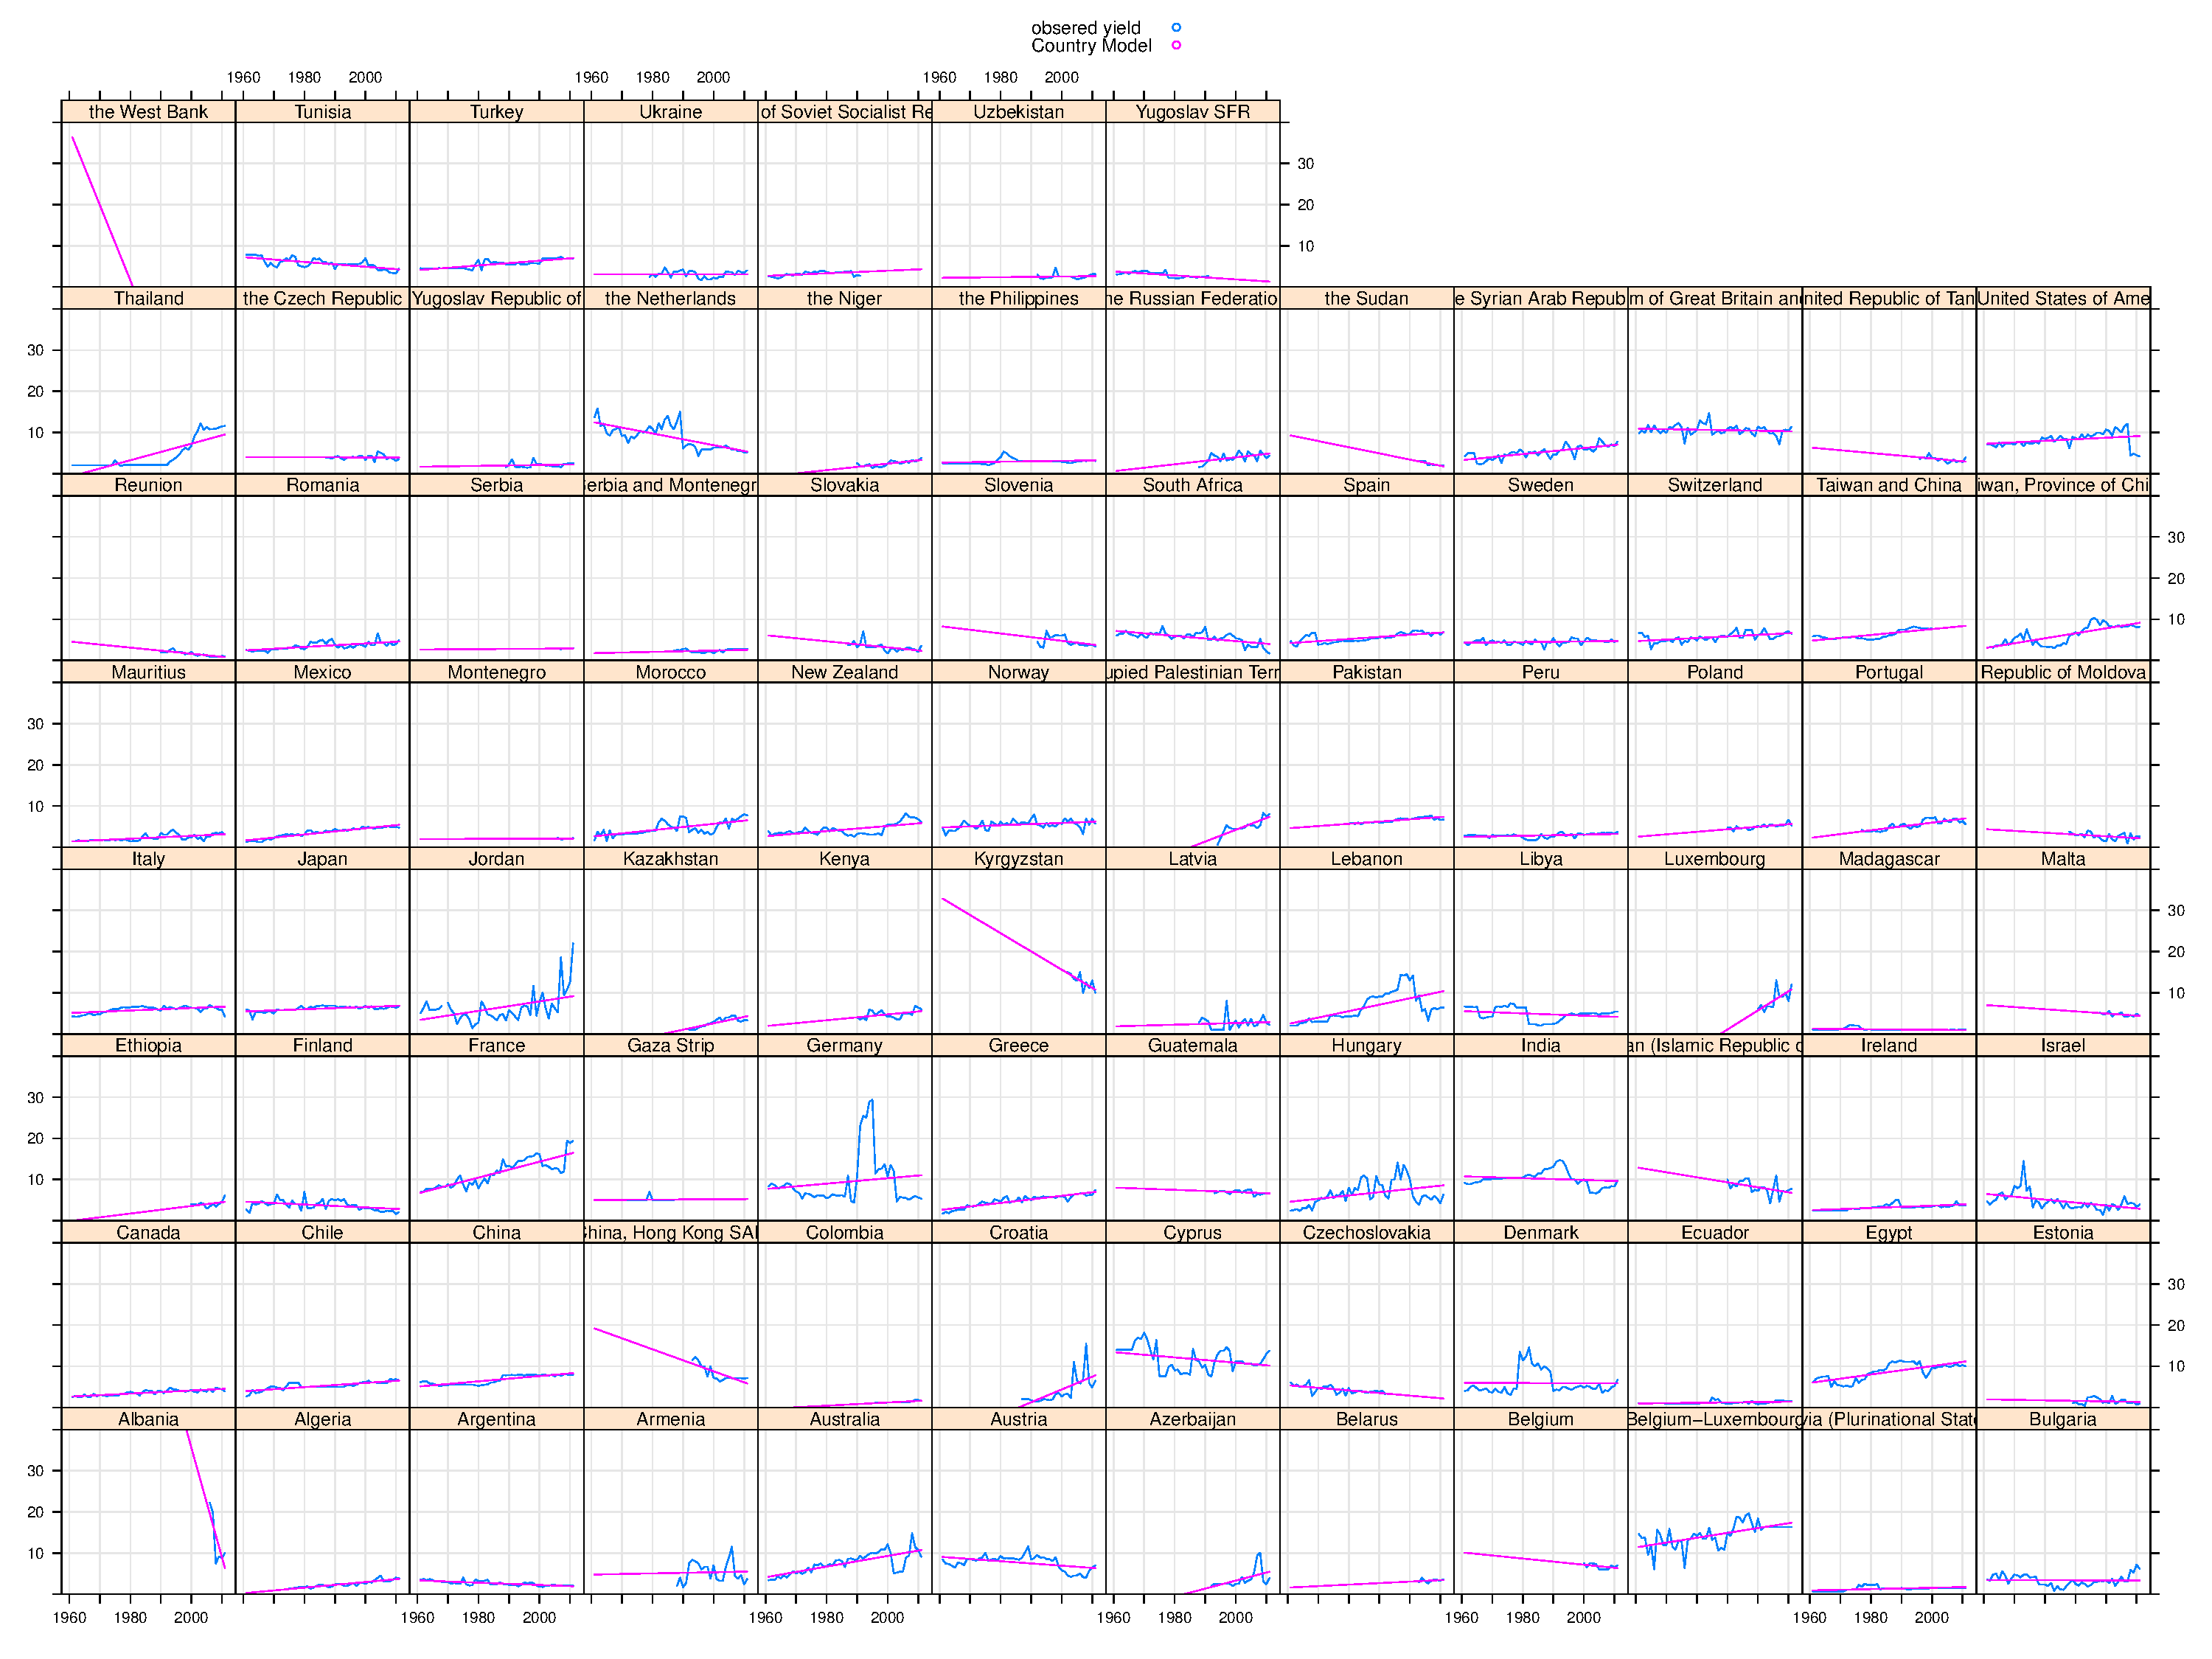
\includegraphics[scale = 0.2]{peasGreenYieldCountry}
}

\frame{
  \frametitle{Linear Mixed Model}
  % Illustrate how the linear mixed model solve the problem shown in
  % the previous two slide.
  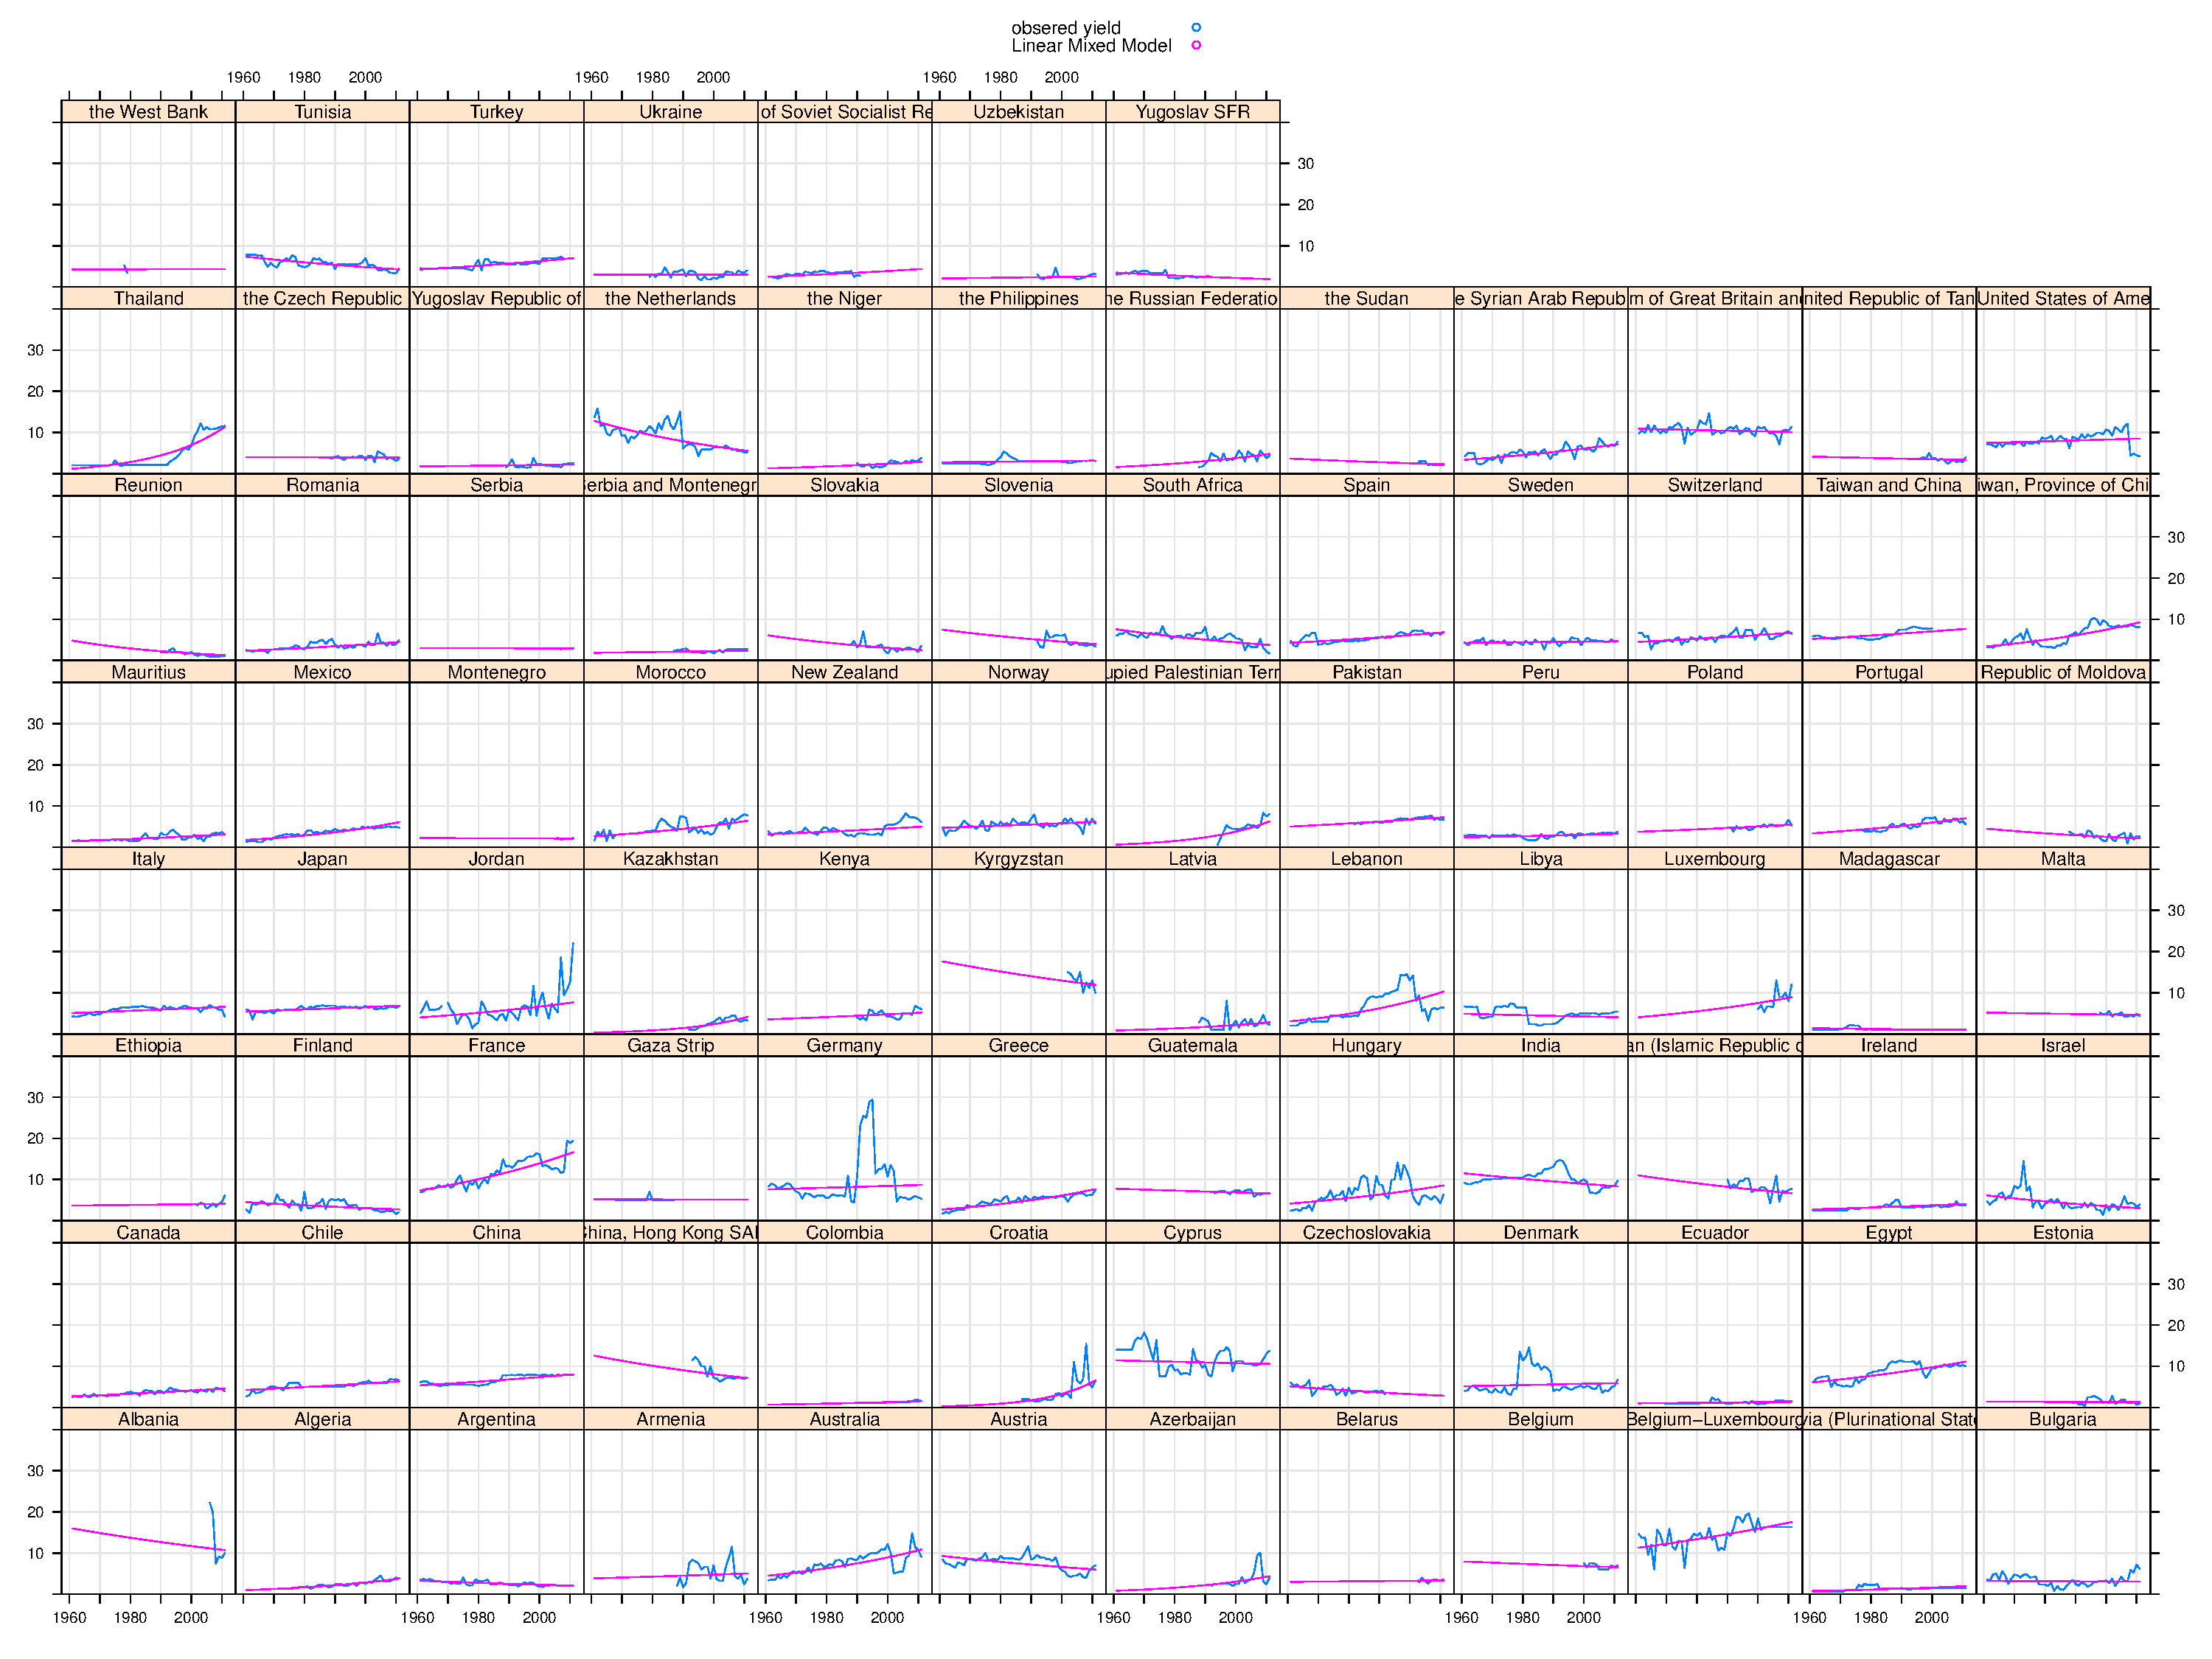
\includegraphics[scale = 0.2]{peasGreenYieldLme}
}

\frame{
  \frametitle{Linear Mixed Model with Splines}
  % Illustrate how the linear mixed model solve the problem shown in
  % the previous two slide.
  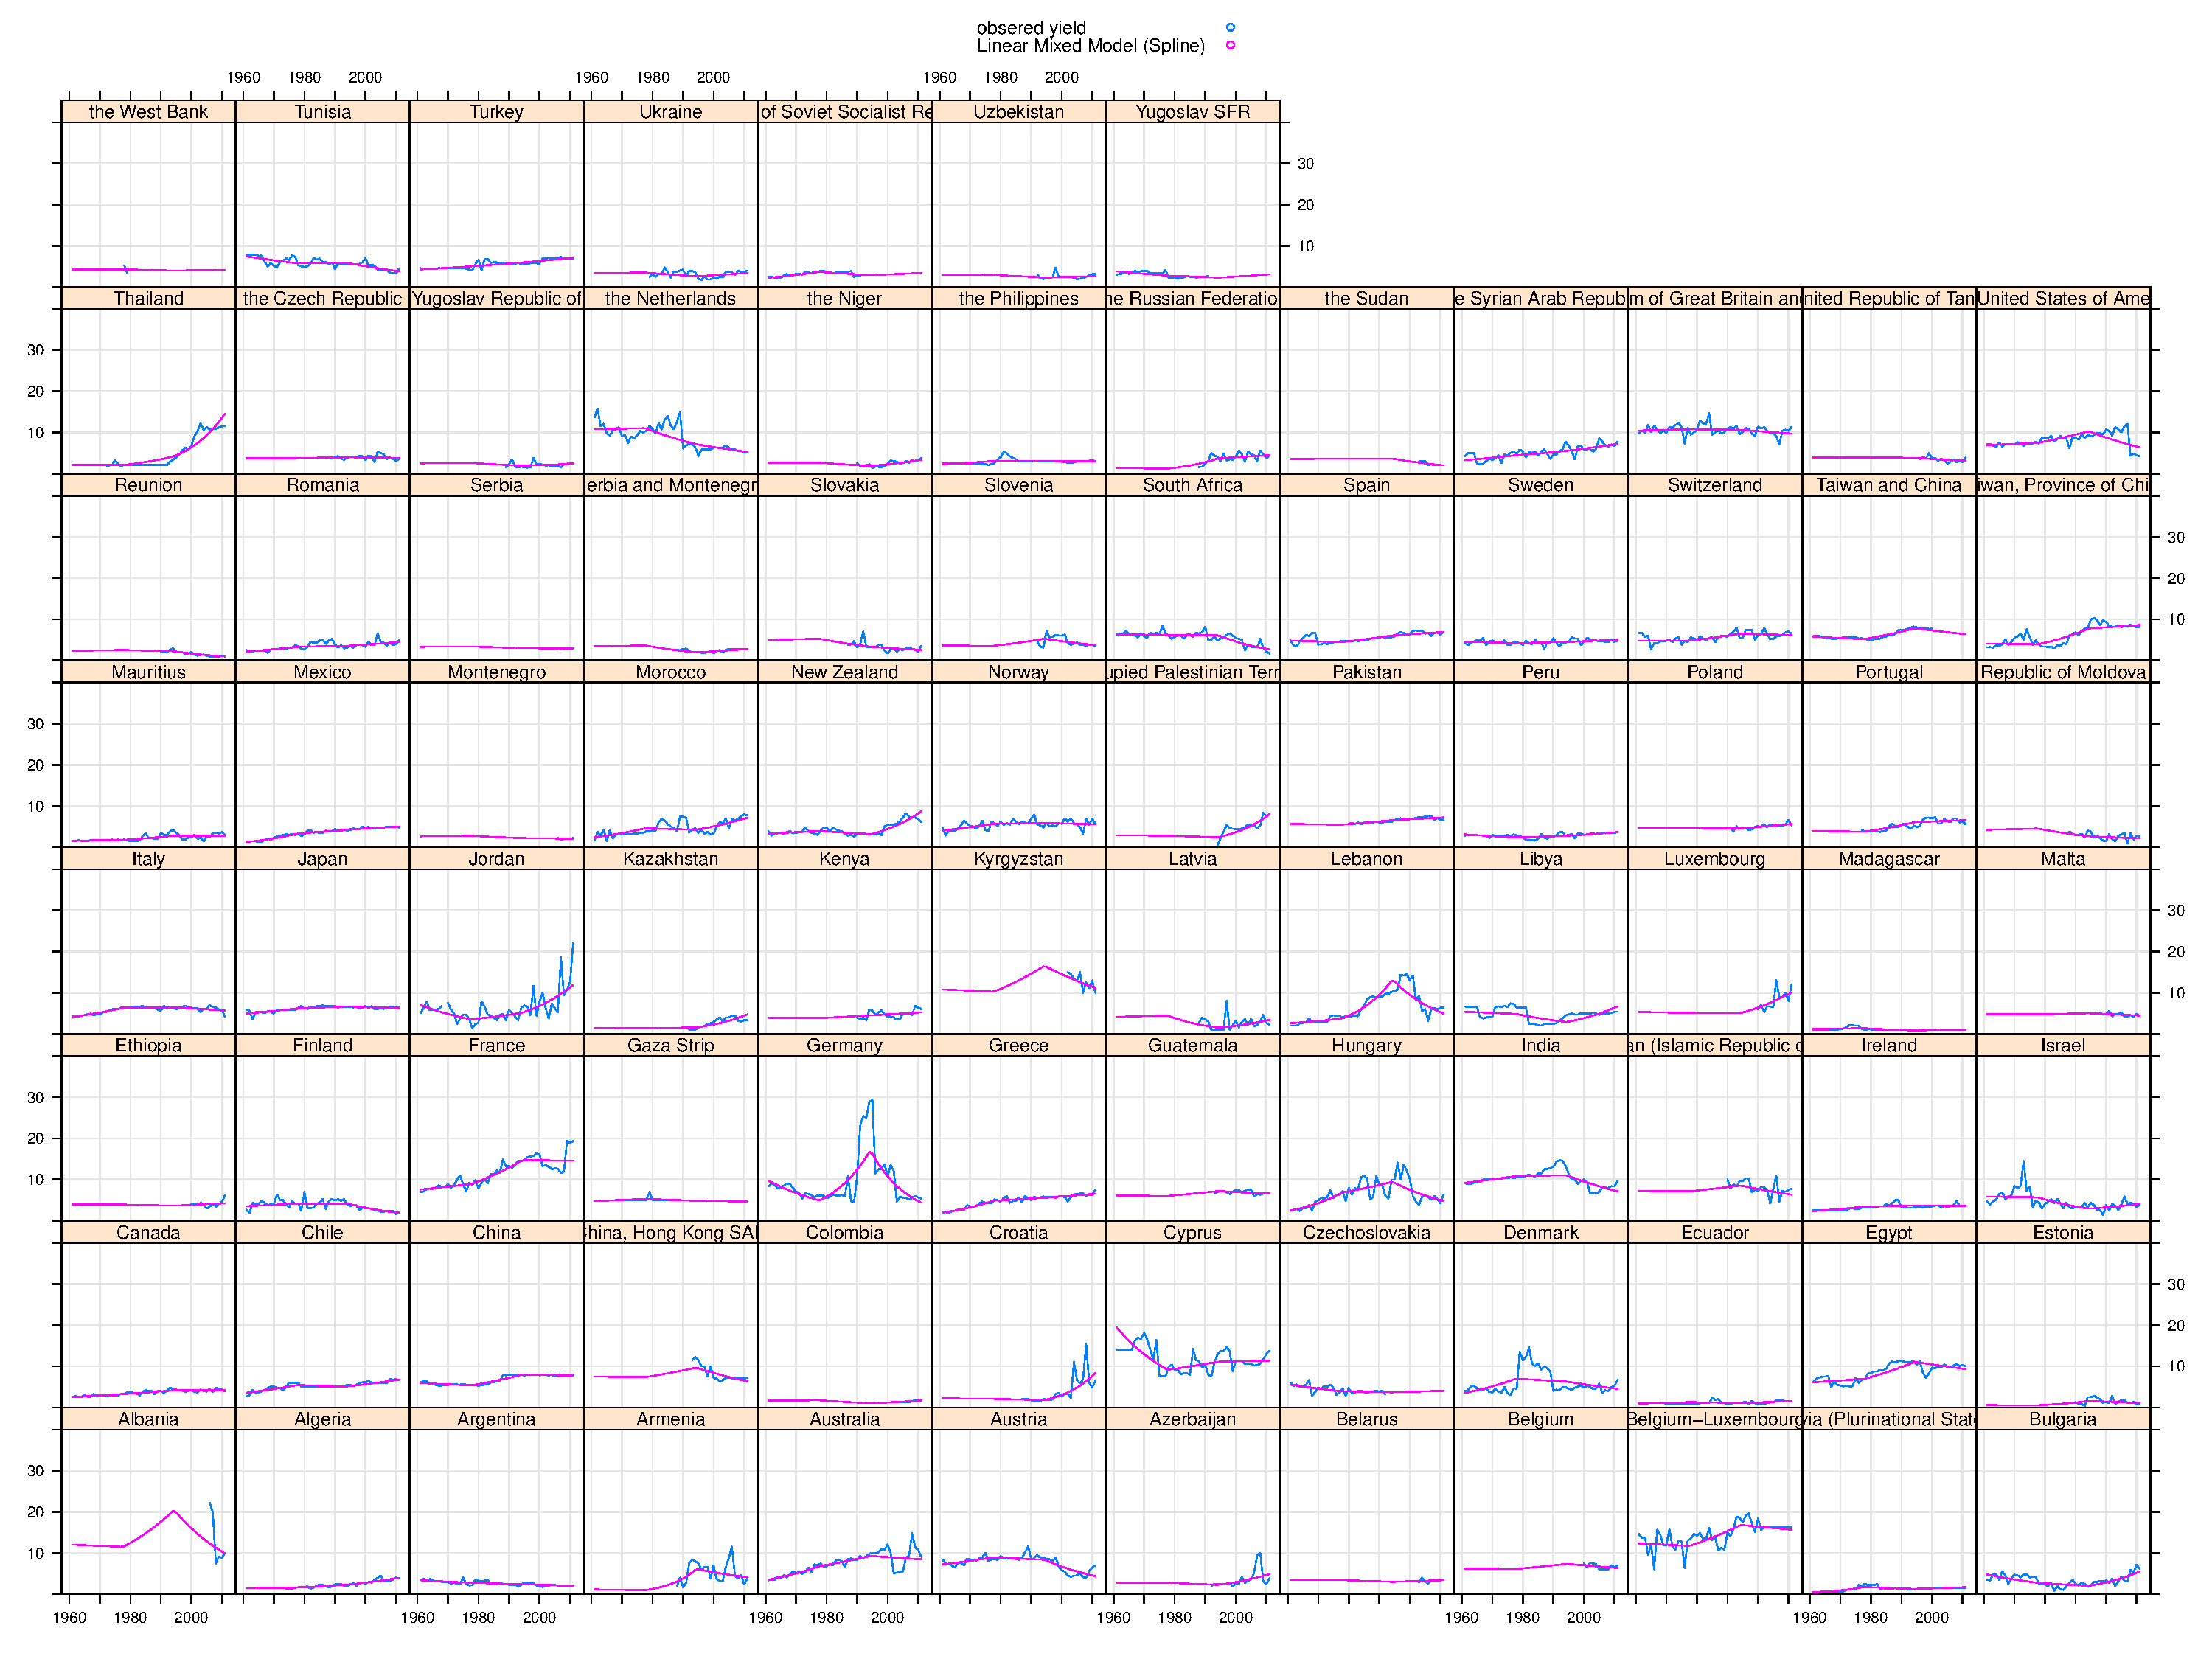
\includegraphics[scale = 0.2]{peasGreenYieldSplineLme}
}



\frame{
  \frametitle{}

  There are several reasons why linear mixed model resolve many
  problems which are associated with fitting a global or country
  level model.

  \vfill

  \begin{itemize}
    \item It utlize cross-country information if it exists.
    \item It captures country specific pattern, but conforms to global
      constraints.
    \item This allow us to fit more flexible models without over-fitting.
  \end{itemize}

  \vfill
  It makes a much more reasonable assumption to our data, countries
  are different but similar.

}

\section{Production and Area Harvested}


\frame{
  \frametitle{}

  After the imputation of the yield, we can balance the area harvested
  or production provided the counter-part exists.

  \vfill

  However, the problem is when both of them are missing.
}


\frame{
  \frametitle{}
  % 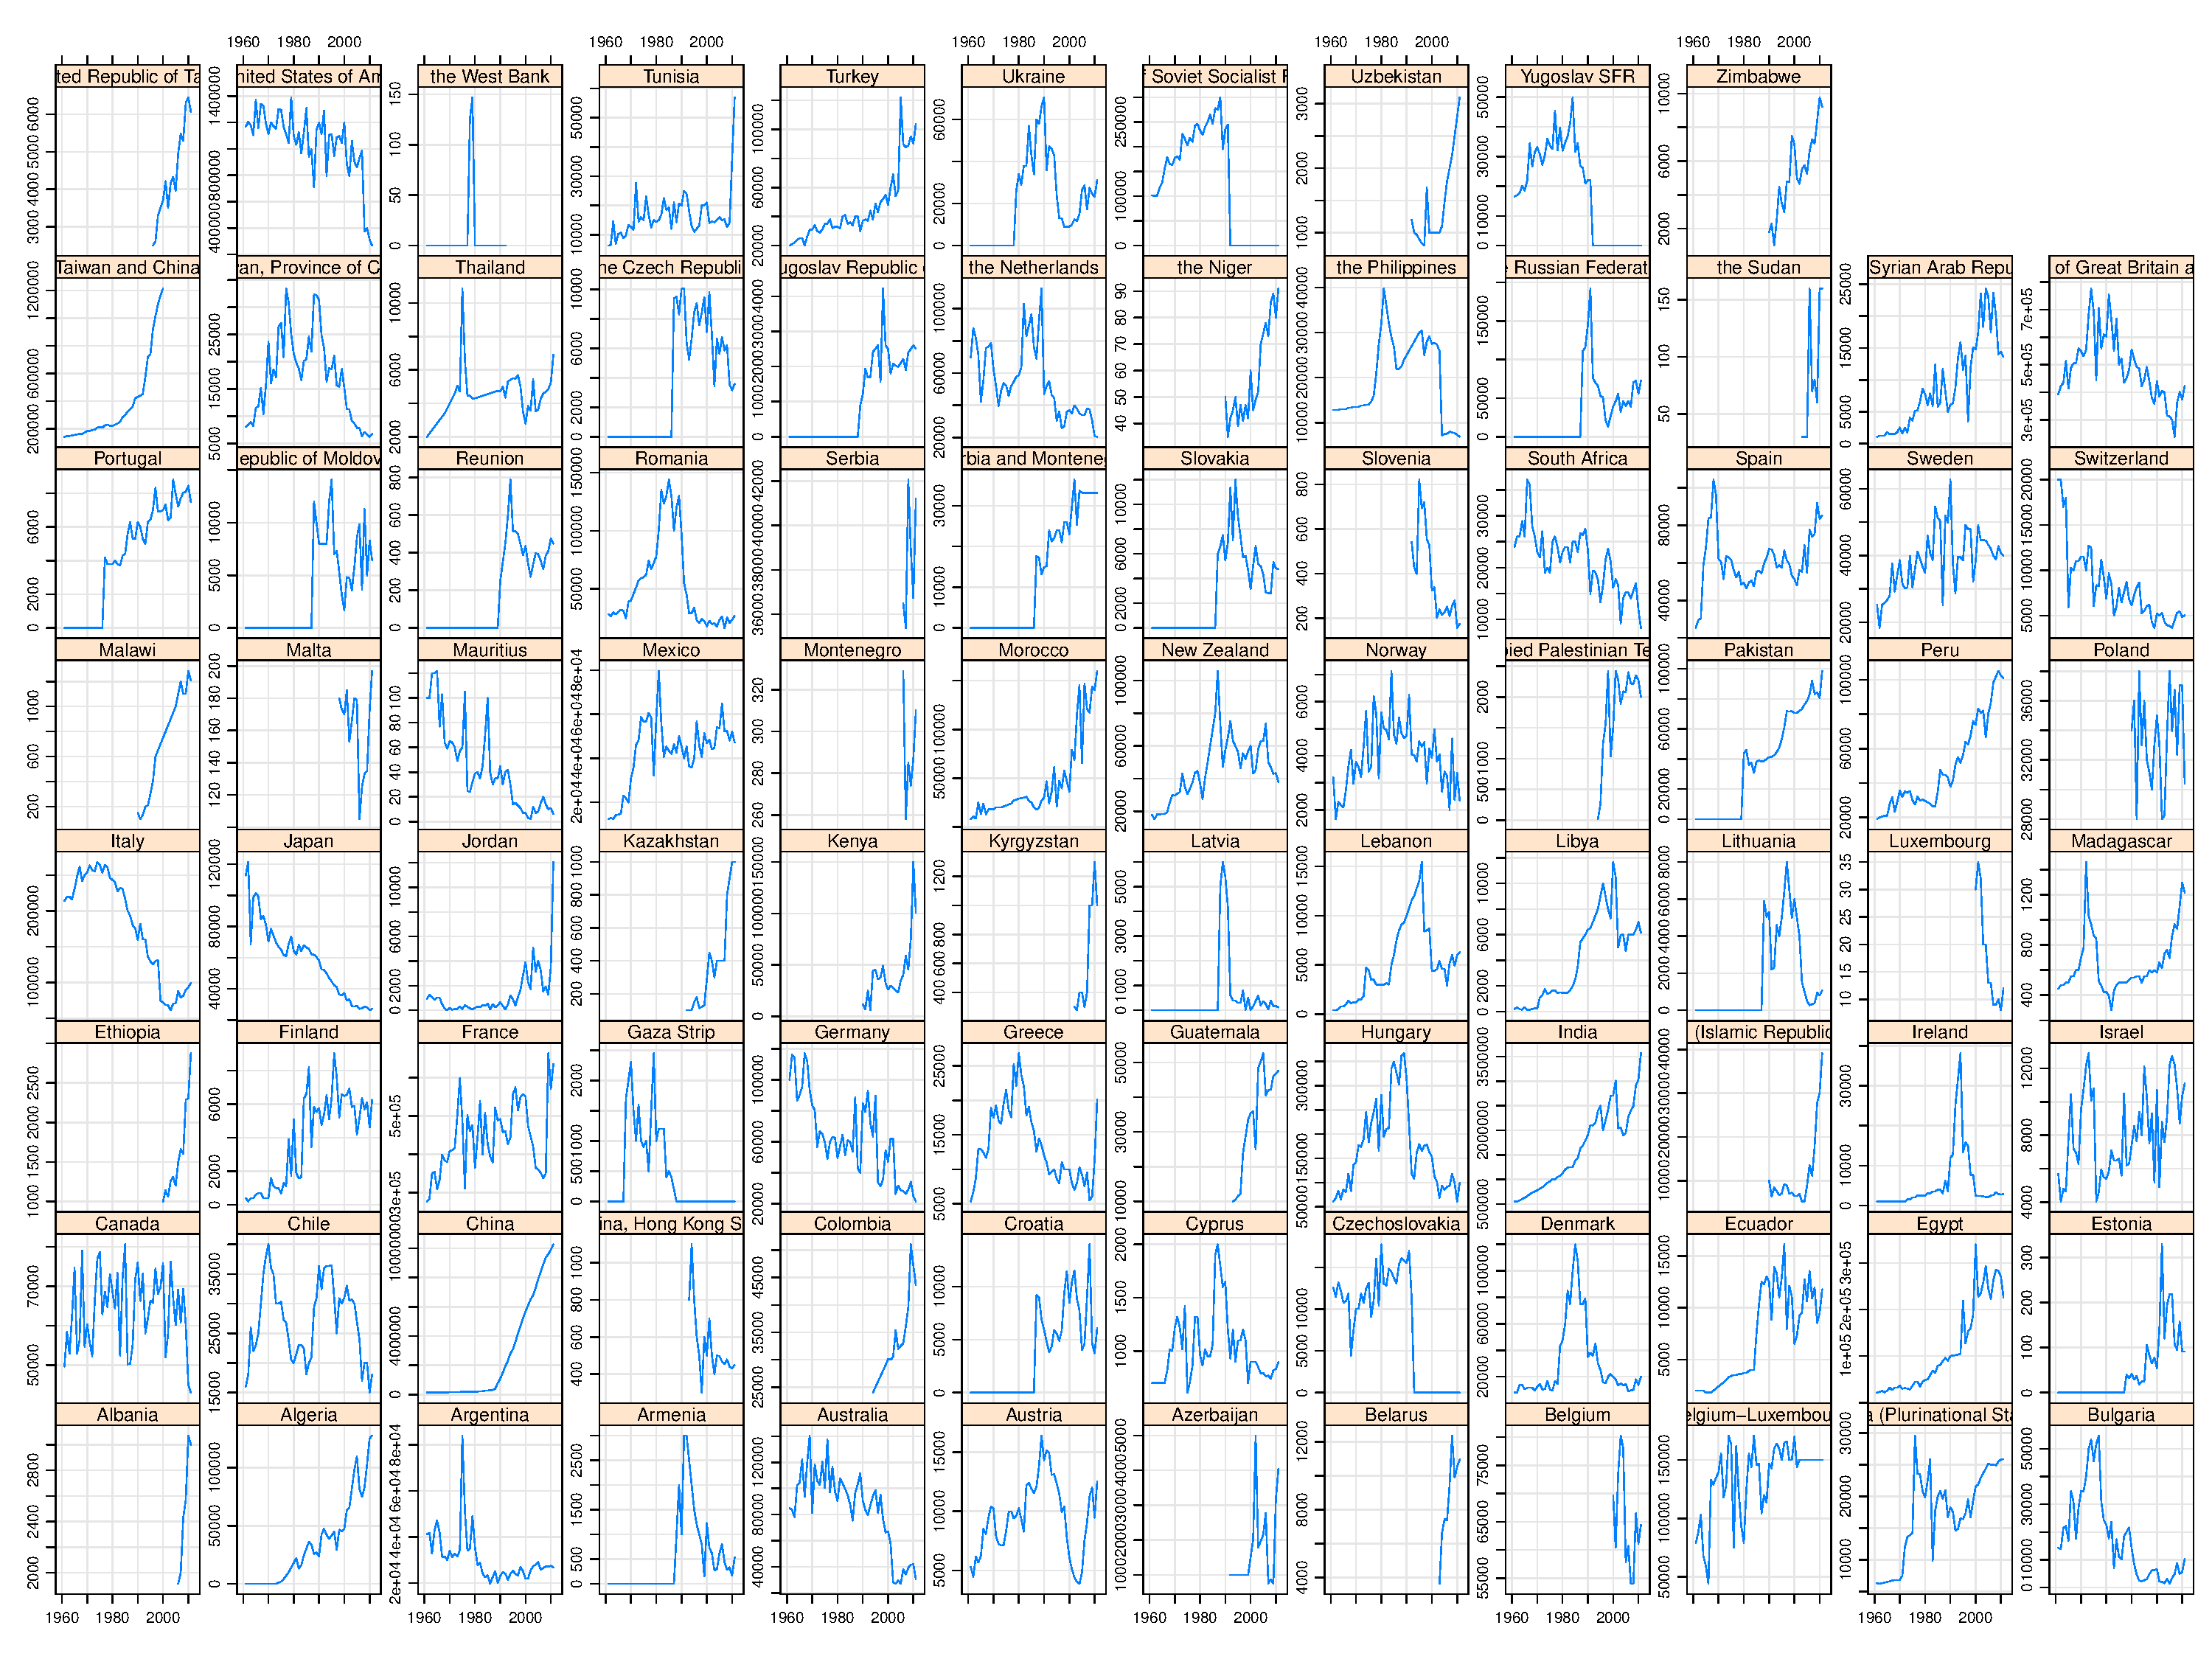
\includegraphics[scale = 0.2]{peasGreenProductionRaw}
  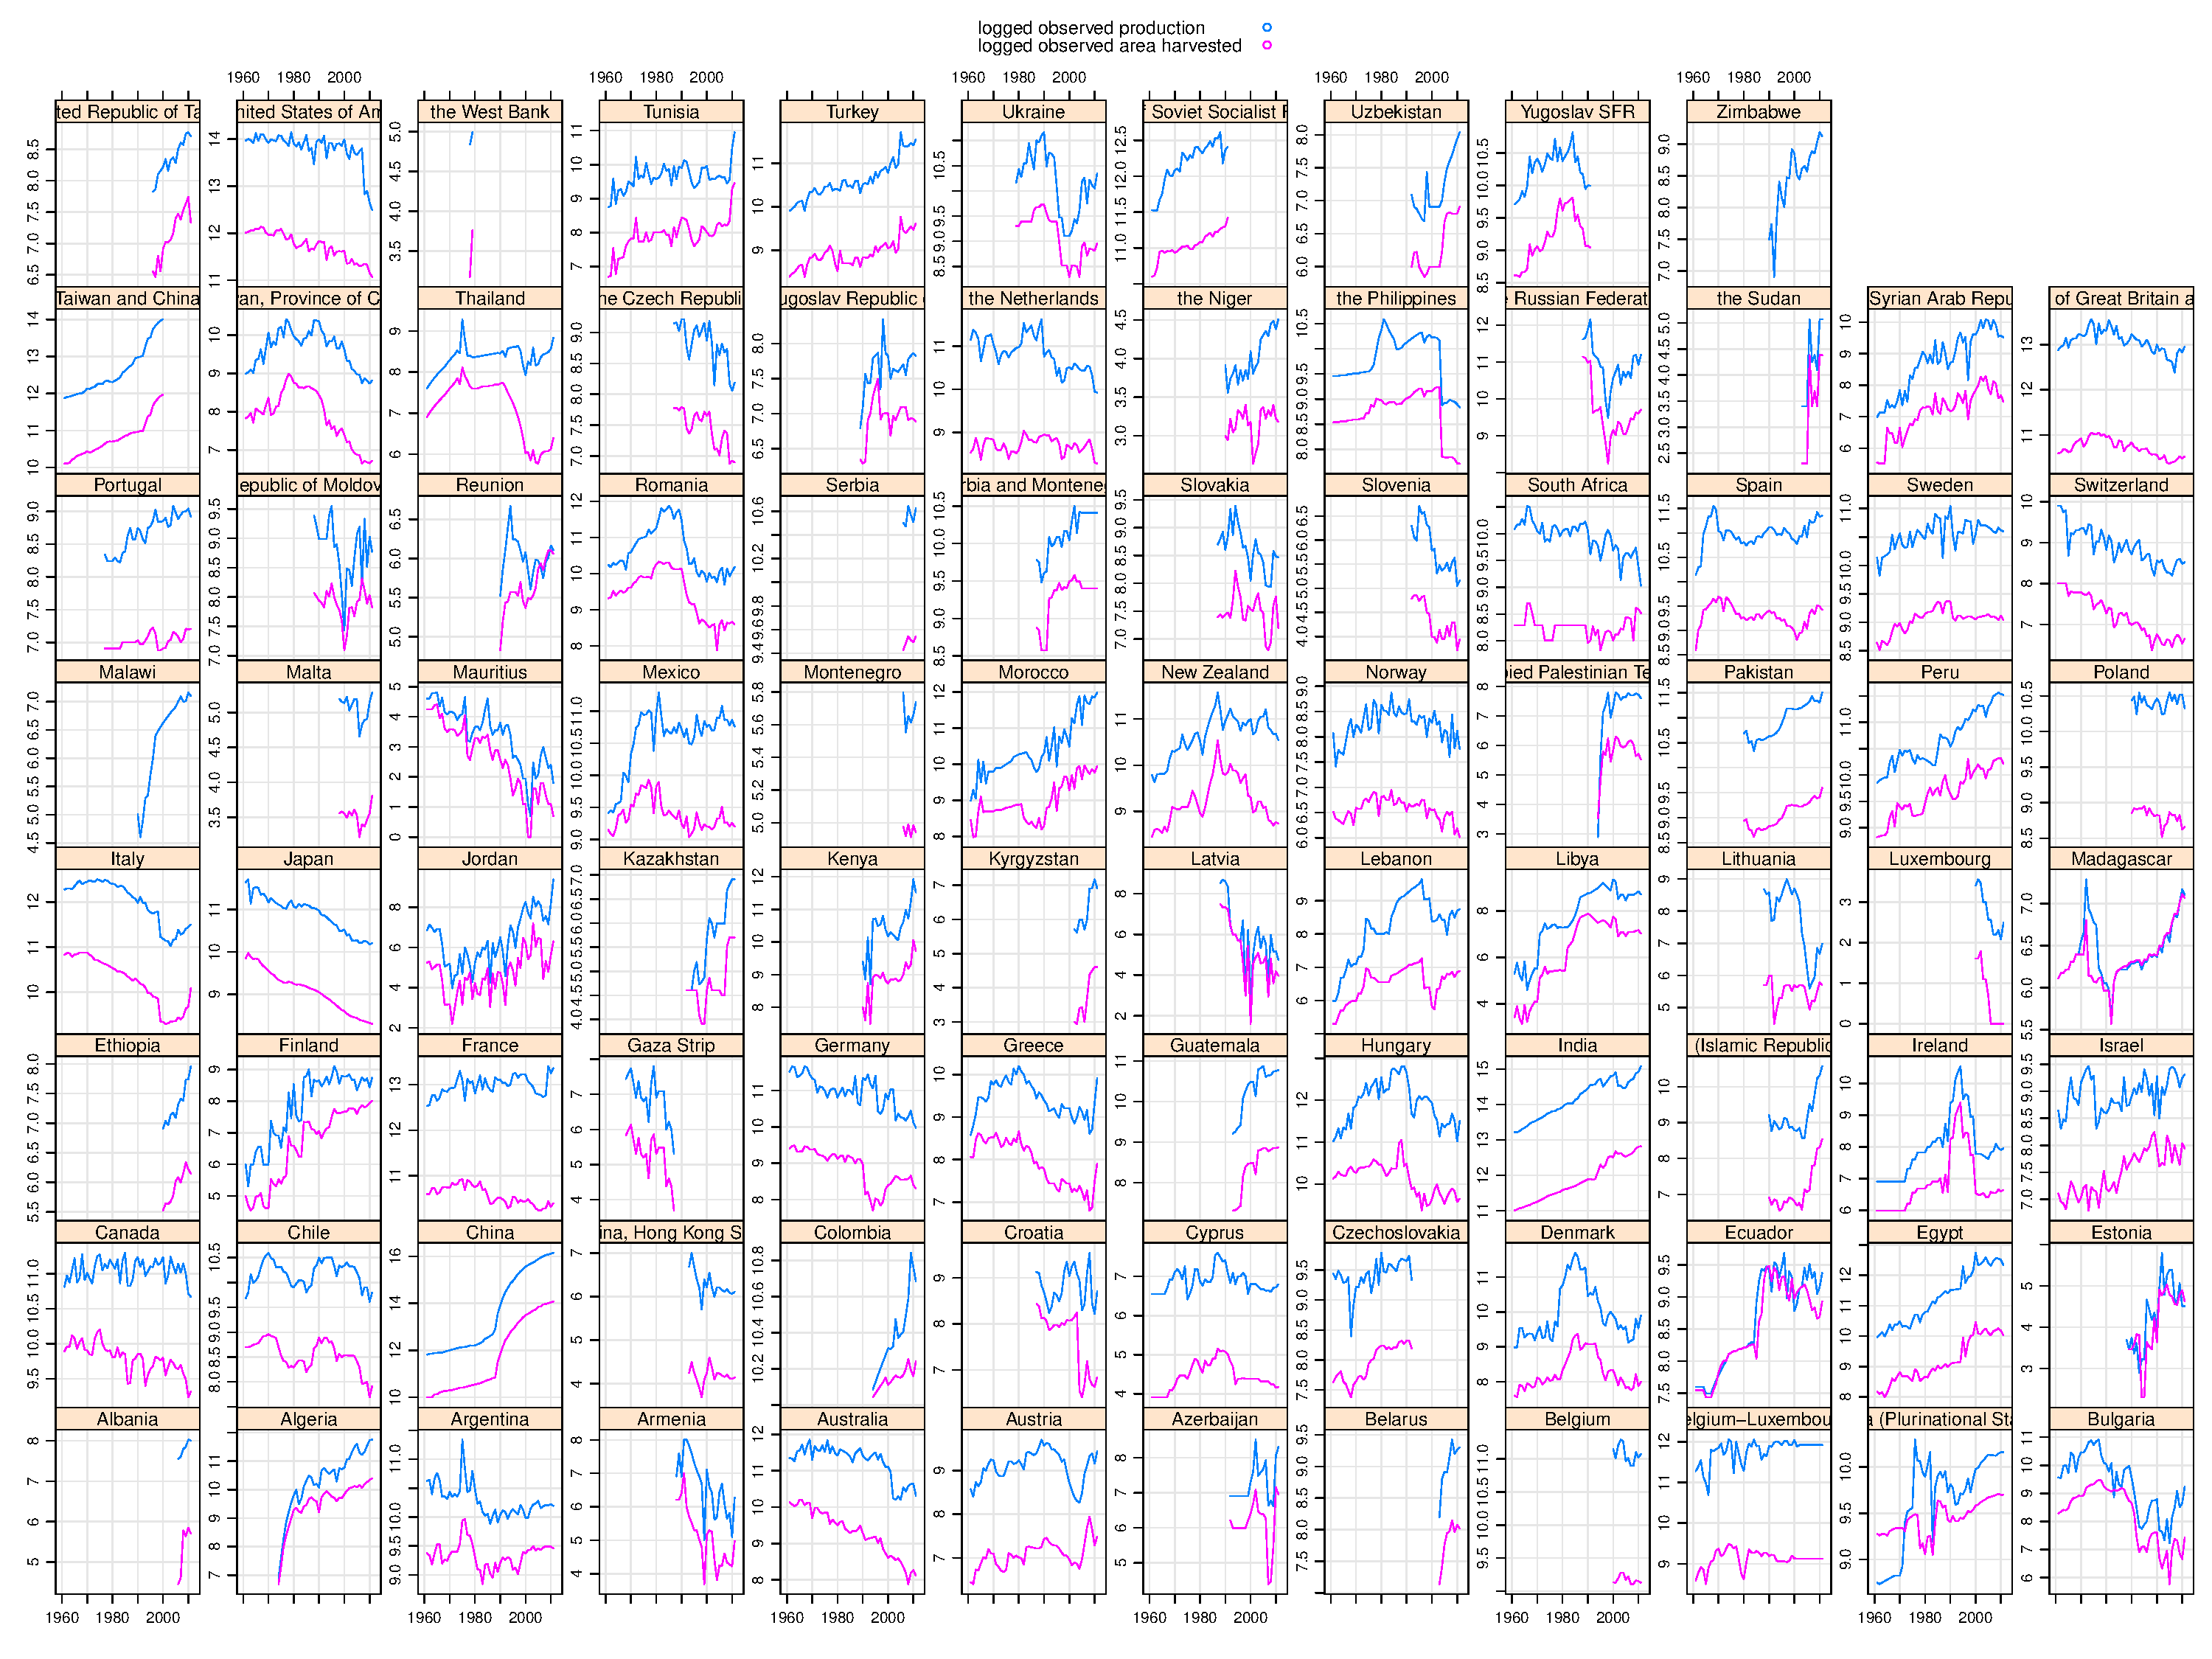
\includegraphics[scale = 0.2]{peasGreenProductionAreaHarvestedRaw}
  % Illustrate the problem that country are very different and that
  % there are no regional information which we can take advantage of.
}



% \frame{
%   \frametitle{}
%   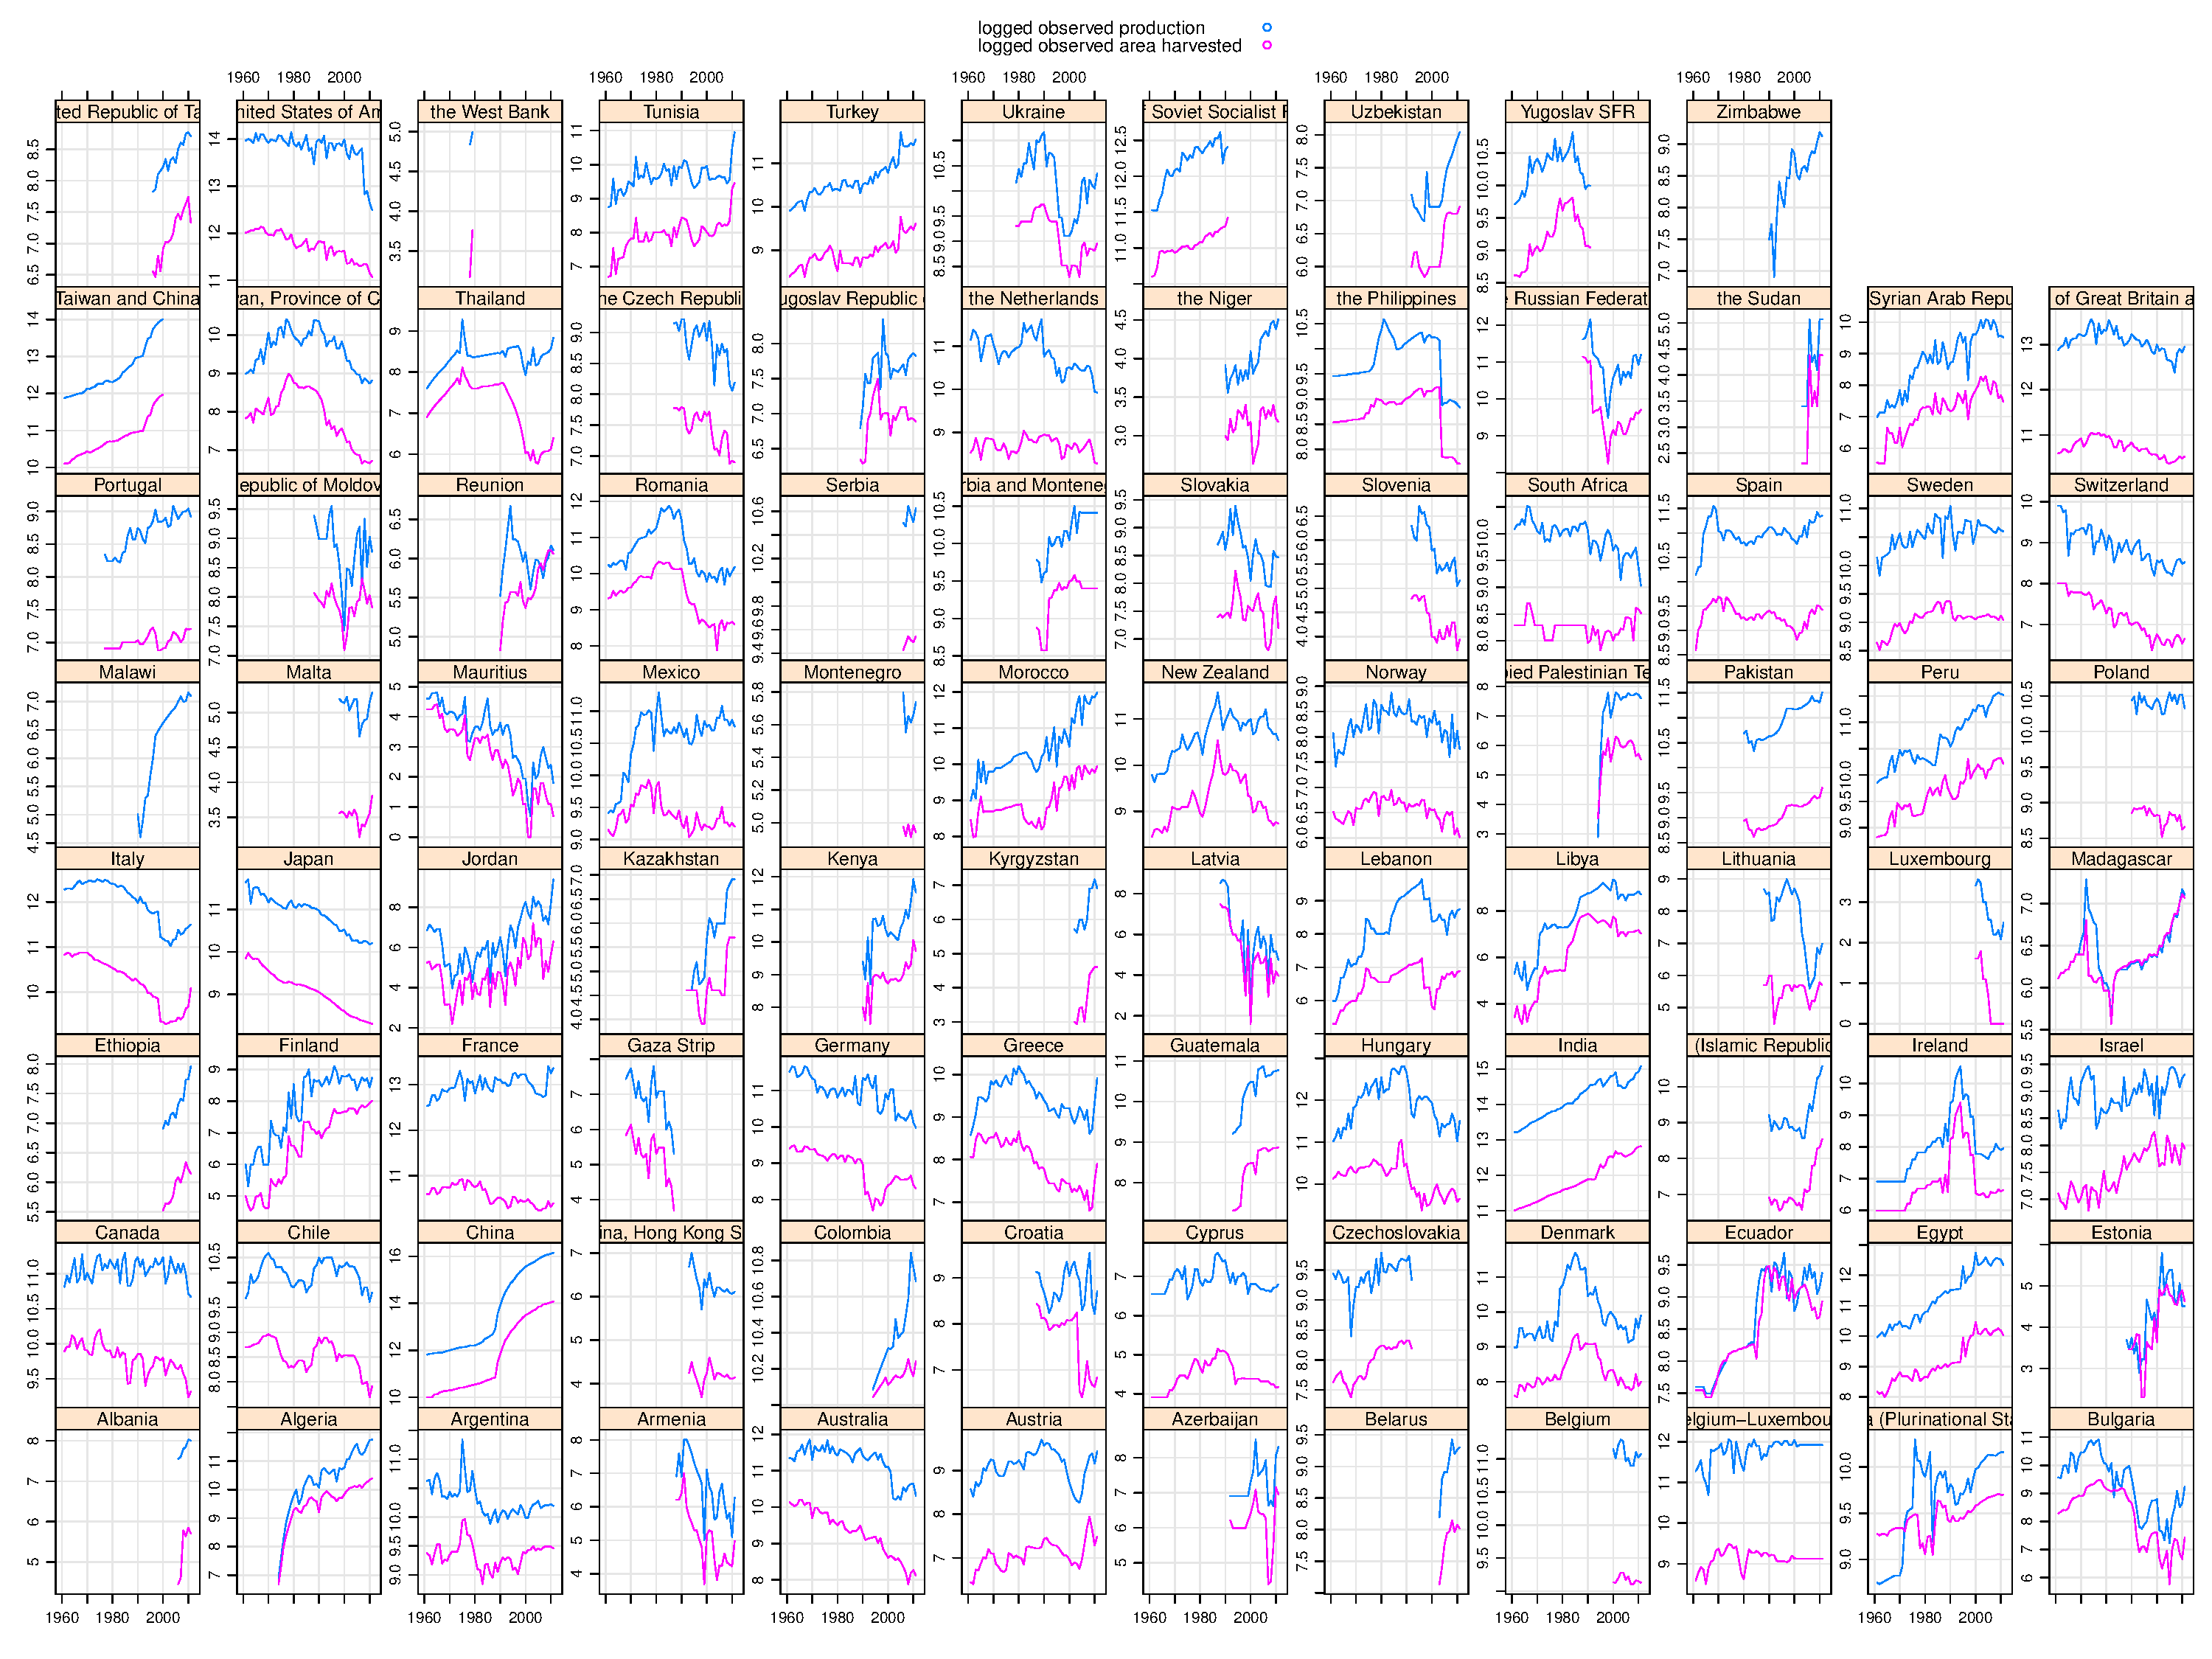
\includegraphics[scale = 0.2]{peasGreenProductionAreaHarvestedRaw}
%   % Illustrate the problem that country are very different and that
%   % there are no regional information which we can take advantage of.
% }

% \frame{
%   \frametitle{}
%   We can see there is a strong linear correlation between production
%   and area harvested.
%   \vfill
%   Which gives us a descent imputation when one of them exist.
%   \vfill
%   However, the core problem exist when both area harvested and
%   production are missing.
% }


\frame{
  \frametitle{What is the solution?}

  Oppose to yield, we have no clear cross-country information which we
  can utilize.

  \vfill

  Furthermore, we actually have no idea about the trend, or even the
  shape of production!

  % Talk about how all time series behave differently, and also at the
  % same time that we may have very small number of observed points
  % for any complex modelling.
}

\frametitle{
  \frametitle{}
  % Plot the production by sub-region
}

\frame{
  \frametitle{}
  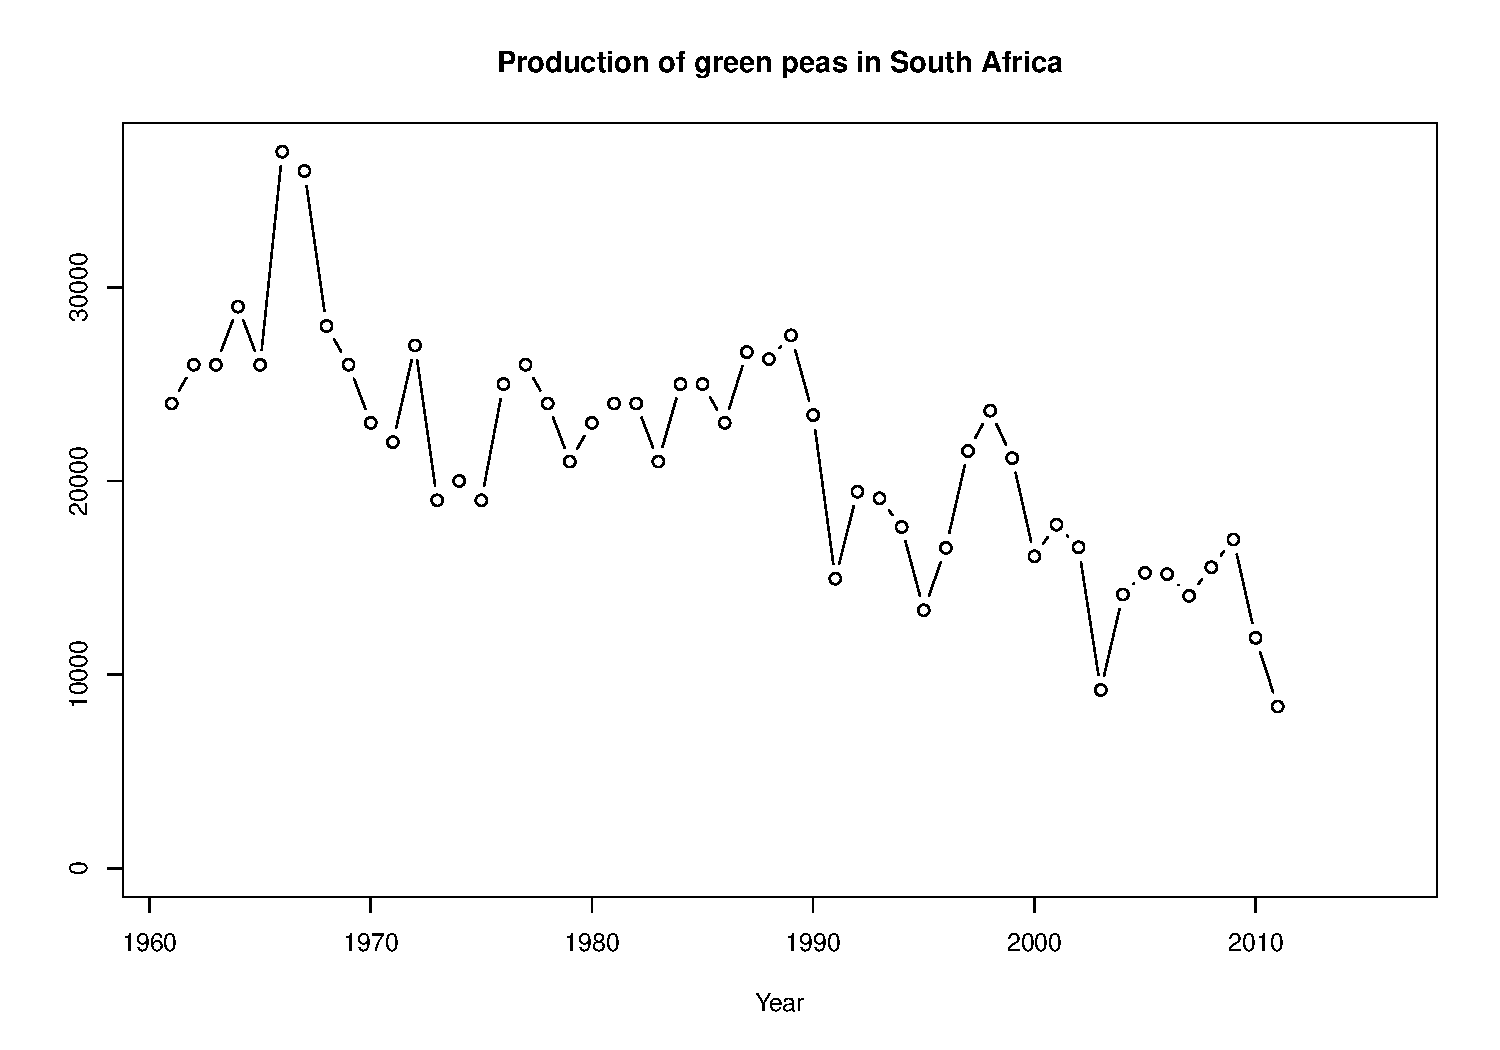
\includegraphics[scale = 0.4, page = 1]{productionEasy}
  %% Give several plots showing the different behaviour of the time
  %% series. (Both production and area harvested)
}

\frame{
  \frametitle{}
  \includegraphics[scale = 0.4, page = 2]{productionEasy}
  %% Give several plots showing the different behaviour of the time
  %% series. (Both production and area harvested)
}

\frame{
  \frametitle{}
  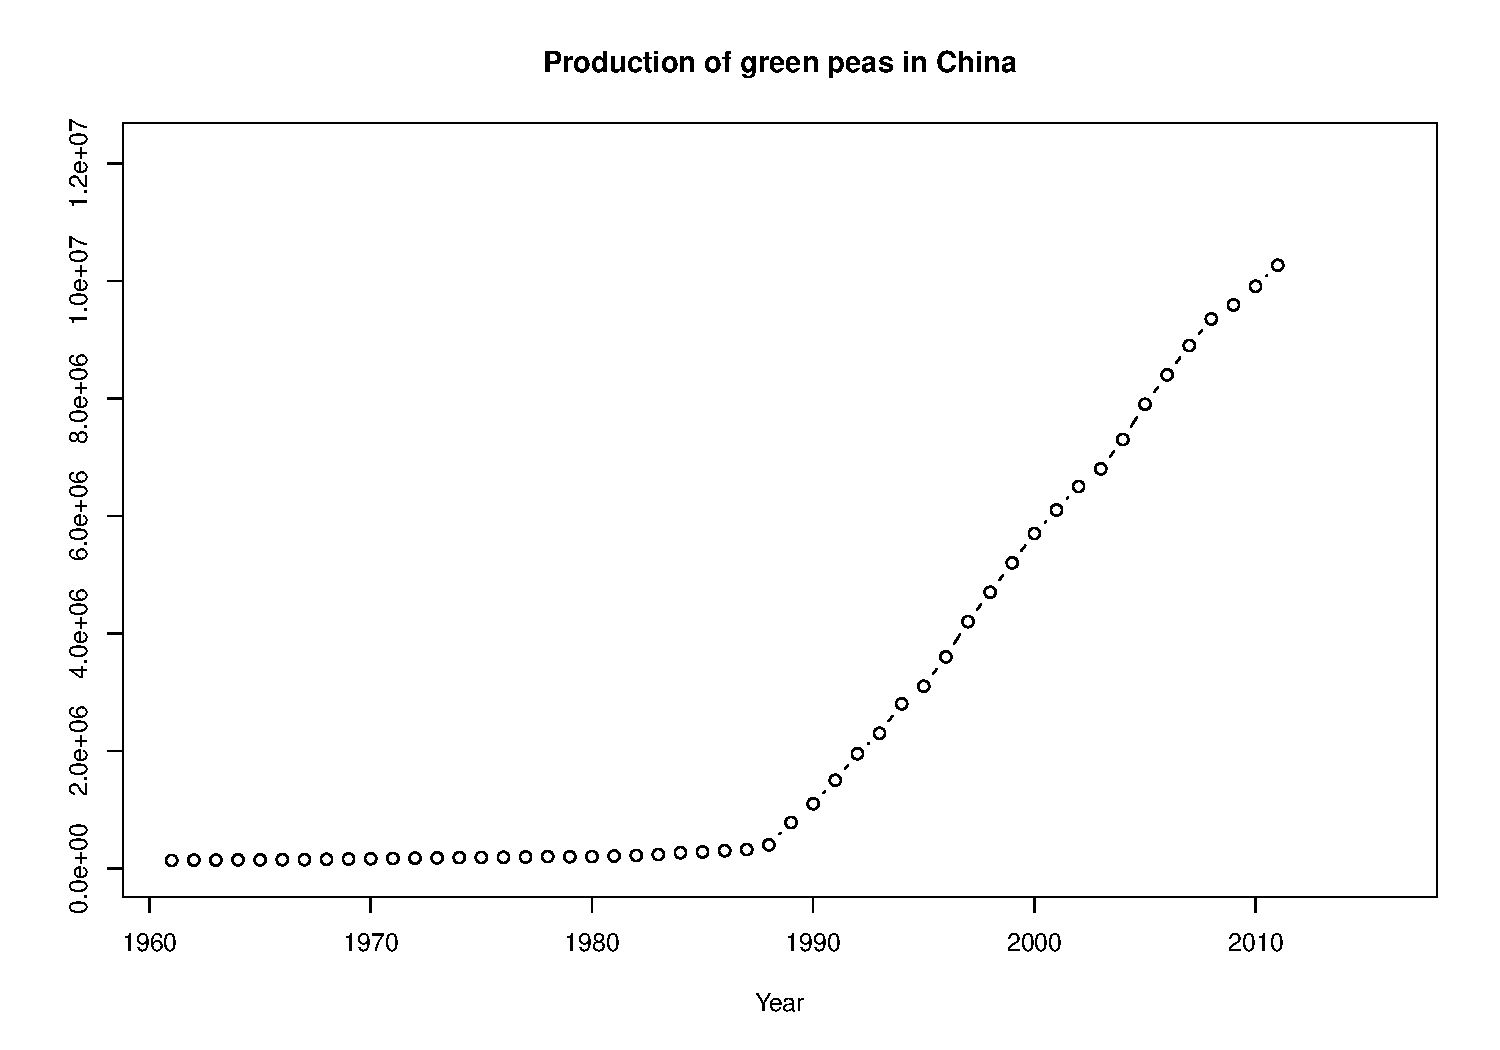
\includegraphics[scale = 0.4, page = 1]{productionModerate}
  %% Give several plots showing the different behaviour of the time
  %% series. (Both production and area harvested)
}

\frame{
  \frametitle{}
  \includegraphics[scale = 0.4, page = 2]{productionModerate}
  %% Give several plots showing the different behaviour of the time
  %% series. (Both production and area harvested)
}


\frame{
  \frametitle{}
  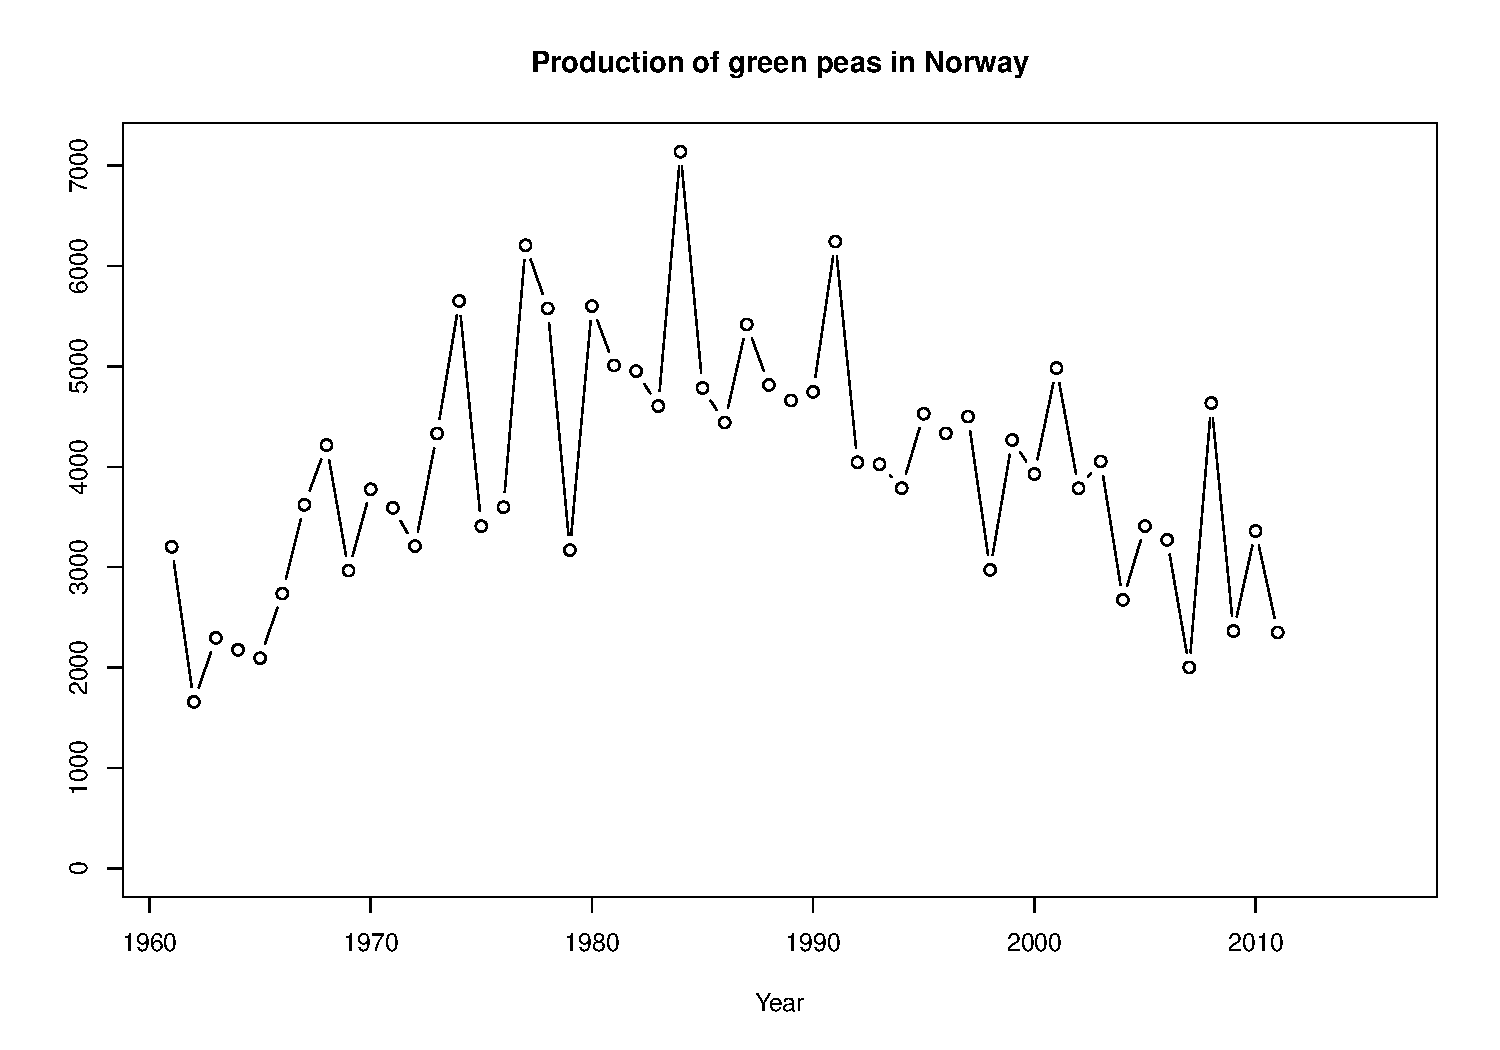
\includegraphics[scale = 0.4, page = 1]{productionDifficult2}
  %% Give several plots showing the different behaviour of the time
  %% series. (Both production and area harvested)
}

\frame{
  \frametitle{}
  \includegraphics[scale = 0.4, page = 2]{productionDifficult2}
  %% Give several plots showing the different behaviour of the time
  %% series. (Both production and area harvested)
}


\frame{
  \frametitle{}
  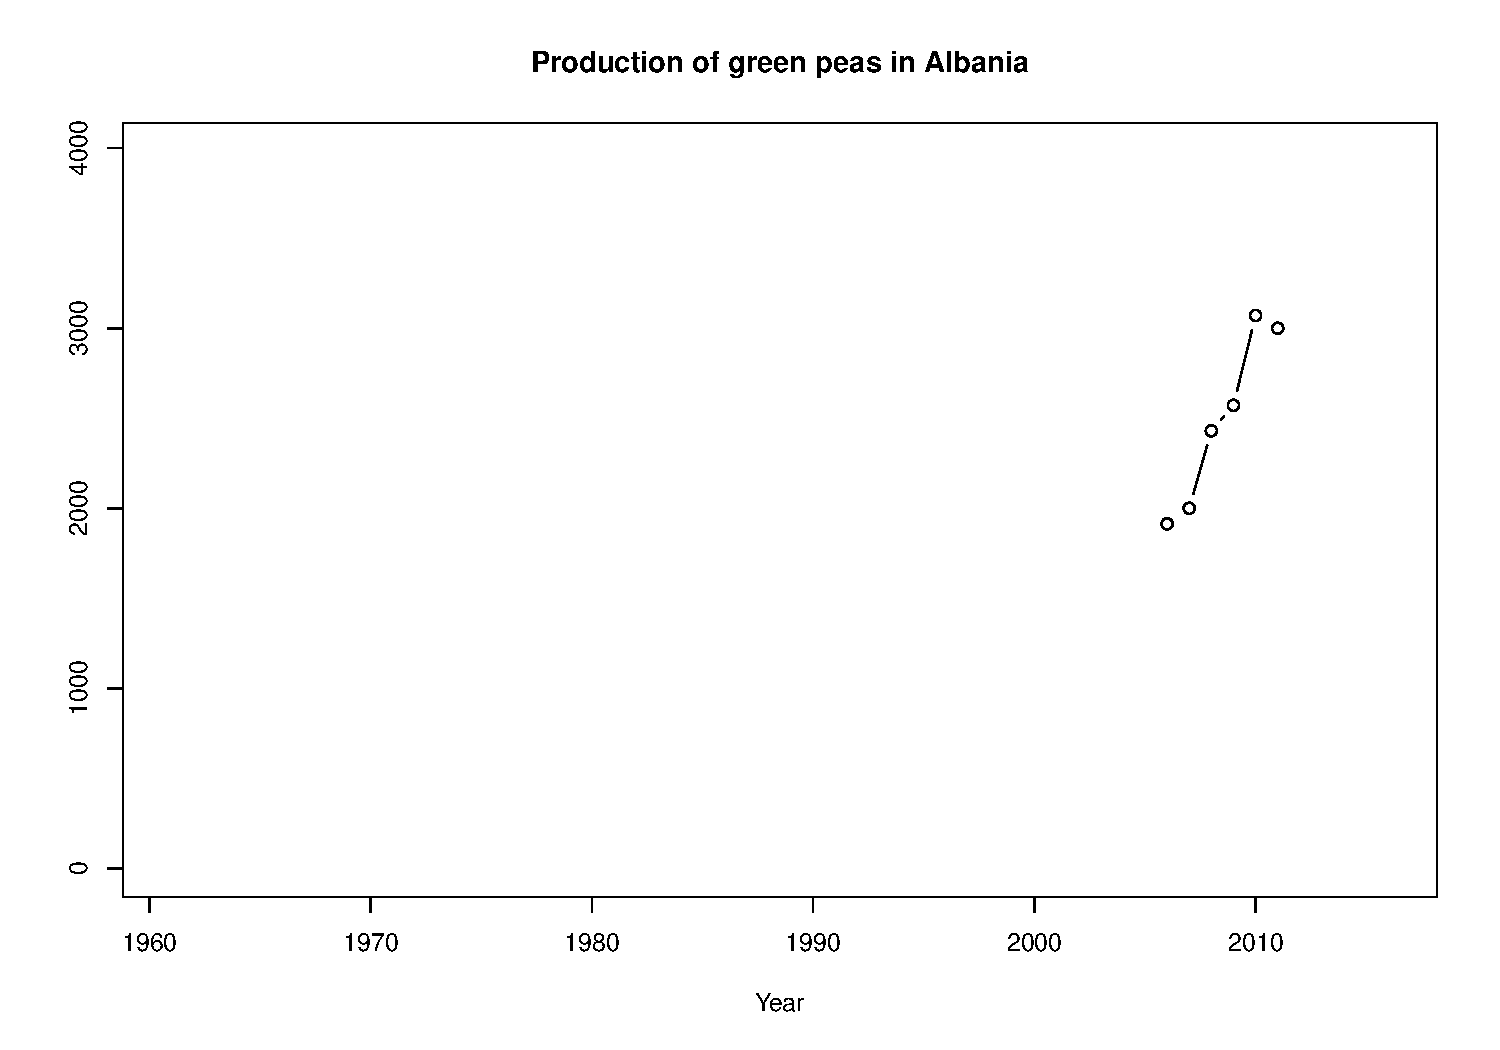
\includegraphics[scale = 0.4, page = 1]{productionDifficult1}
  %% Give several plots showing the different behaviour of the time
  %% series. (Both production and area harvested)
}

\frame{
  \frametitle{}
  \includegraphics[scale = 0.4, page = 2]{productionDifficult1}
  %% Give several plots showing the different behaviour of the time
  %% series. (Both production and area harvested)
}



\frame{
  \frametitle{}
  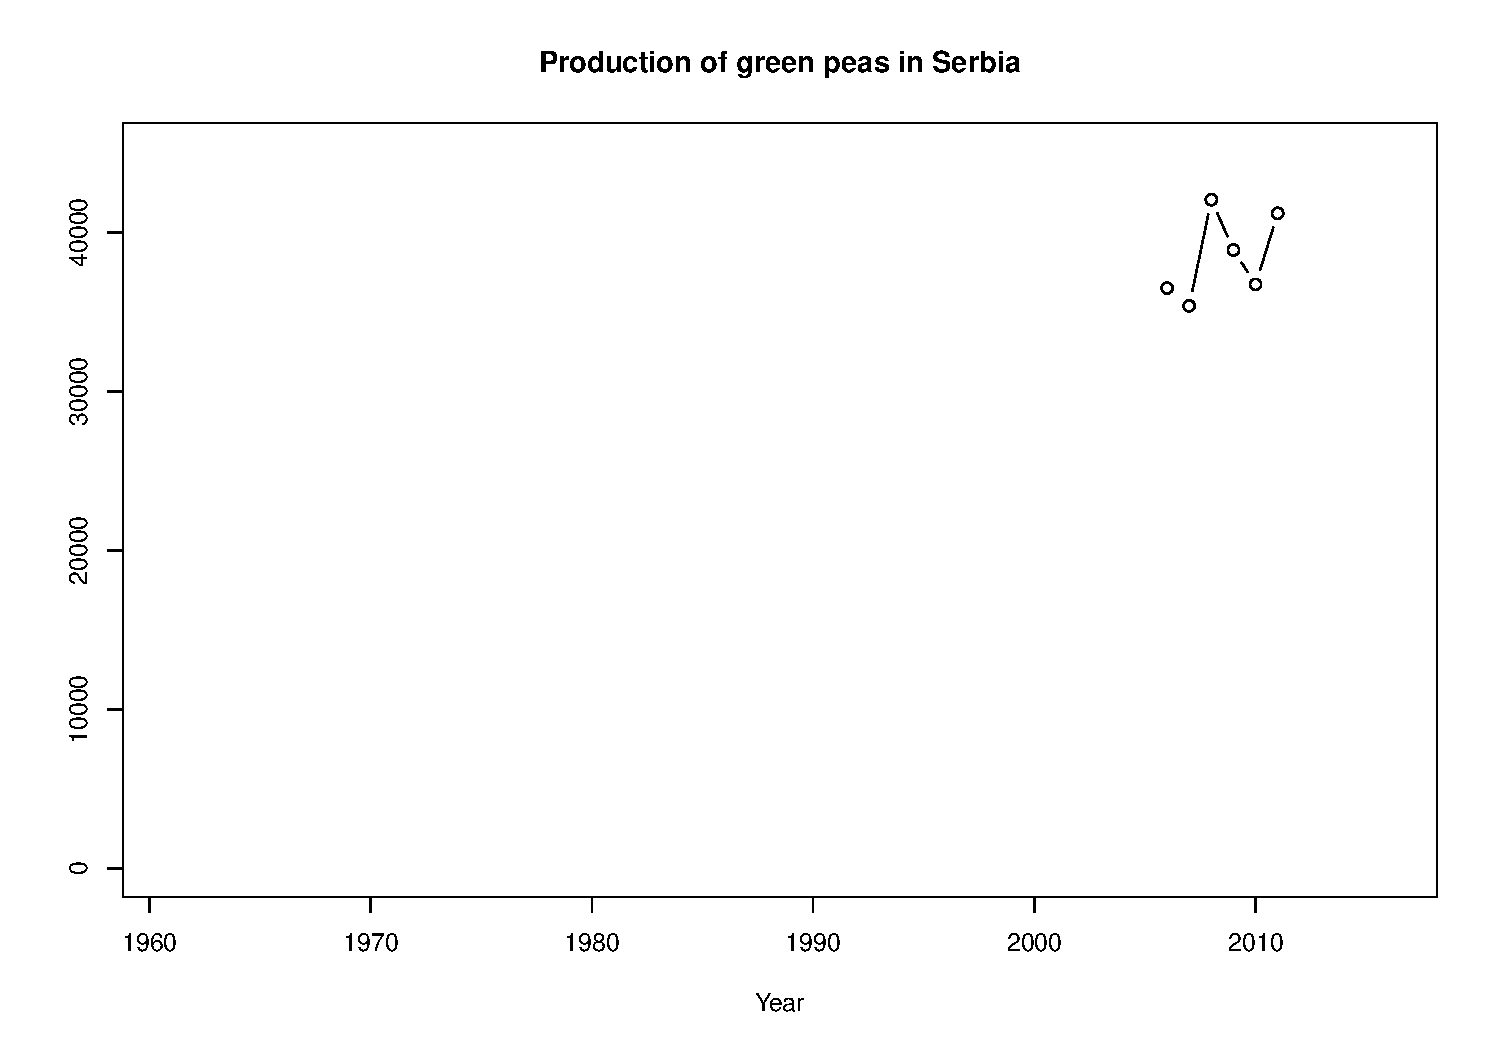
\includegraphics[scale = 0.4, page = 1]{productionHard1}
  %% Give several plots showing the different behaviour of the time
  %% series. (Both production and area harvested)
}

\frame{
  \frametitle{}
  \includegraphics[scale = 0.4, page = 2]{productionHard1}
  %% Give several plots showing the different behaviour of the time
  %% series. (Both production and area harvested)
}

\frame{
  \frametitle{}
  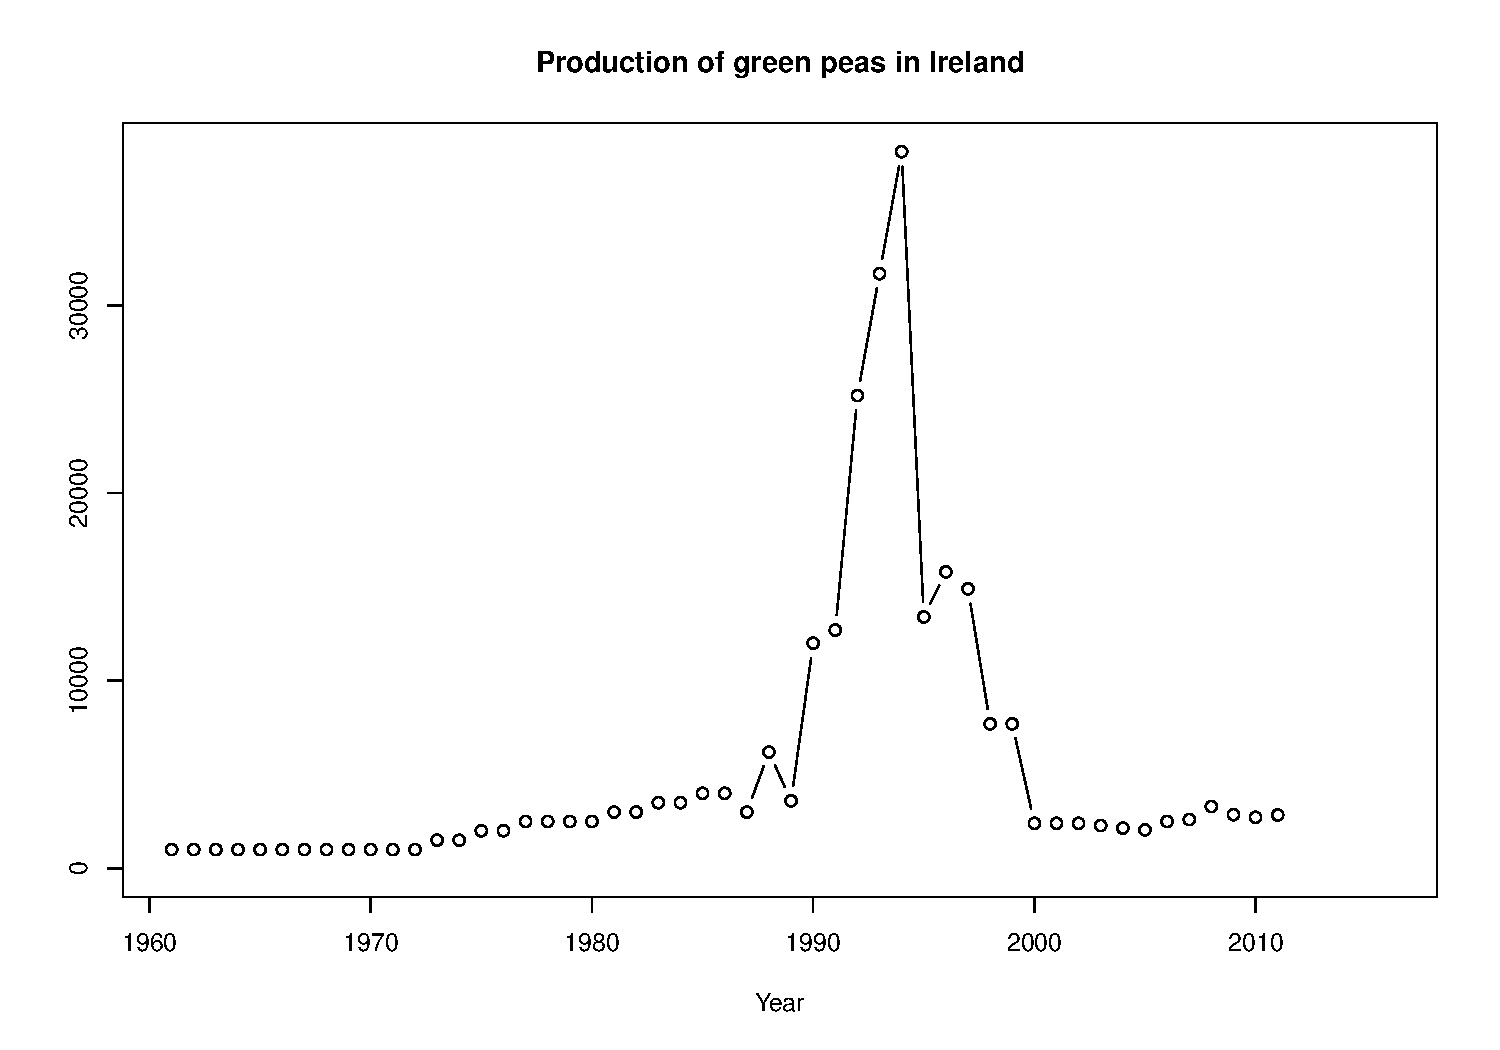
\includegraphics[scale = 0.4, page = 1]{productionHard2}
  %% Give several plots showing the different behaviour of the time
  %% series. (Both production and area harvested)
}

\frame{
  \frametitle{}
  \includegraphics[scale = 0.4, page = 2]{productionHard2}
  %% Give several plots showing the different behaviour of the time
  %% series. (Both production and area harvested)
}


\frame{
  \frametitle{}
  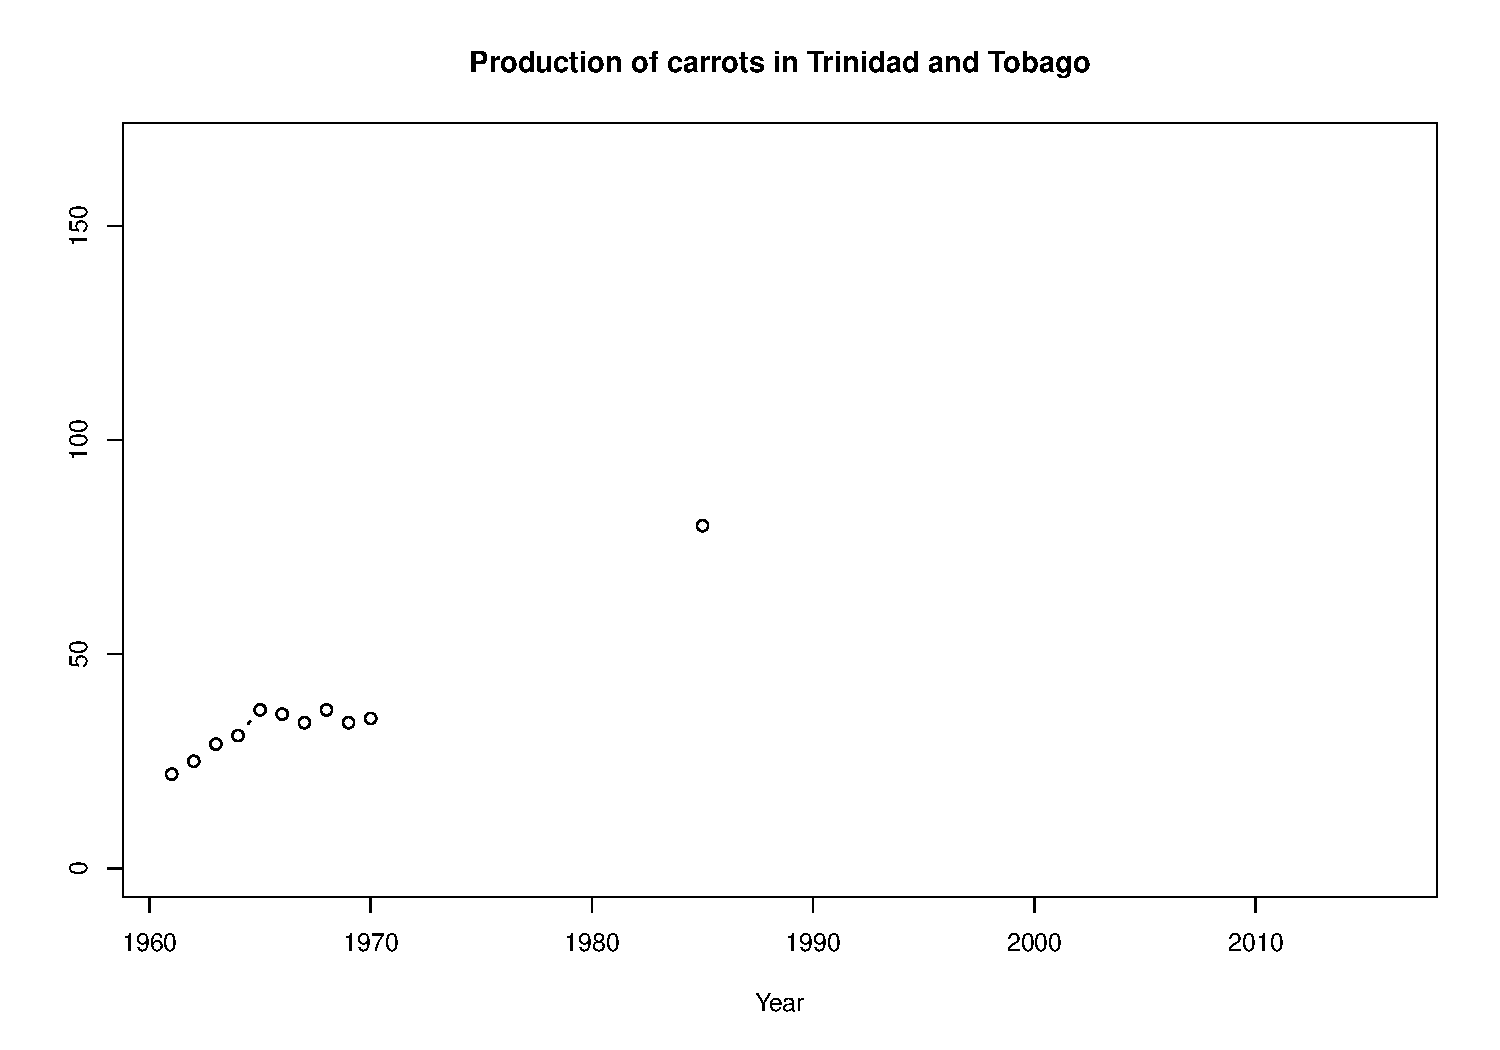
\includegraphics[scale = 0.4, page = 1]{productionImpossible}
  %% Give several plots showing the different behaviour of the time
  %% series. (Both production and area harvested)
}

\frame{
  \frametitle{}
  \includegraphics[scale = 0.4, page = 2]{productionImpossible}
  %% Give several plots showing the different behaviour of the time
  %% series. (Both production and area harvested)
}


\frame{
  \frametitle{What is Ensemble Learning?}

  Ensemble learning in its simplest sense, is to build multiple
  models/learners and combine them to obtain the final model or
  prediction.

  \vfill

  It consist of two components:
  \begin{enumerate}
    \item Building multiple models or learners.
    \item Combine the models and predictions.
  \end{enumerate}

}


\frame{
  \frametitle{Why Ensemble Learning?}

  Ensemble as described by Dietterich (2000) can mitigate the following
  three issues.

  \vfill

  \begin{itemize}
    \setlength{\itemindent}{1in}
    \item[Statistical:] Lack of data to identify an unique solution.
    \item[Computational:] Optimization
    \item[Representational:] Complex model
  \end{itemize}

}

\frame{
  \centering
  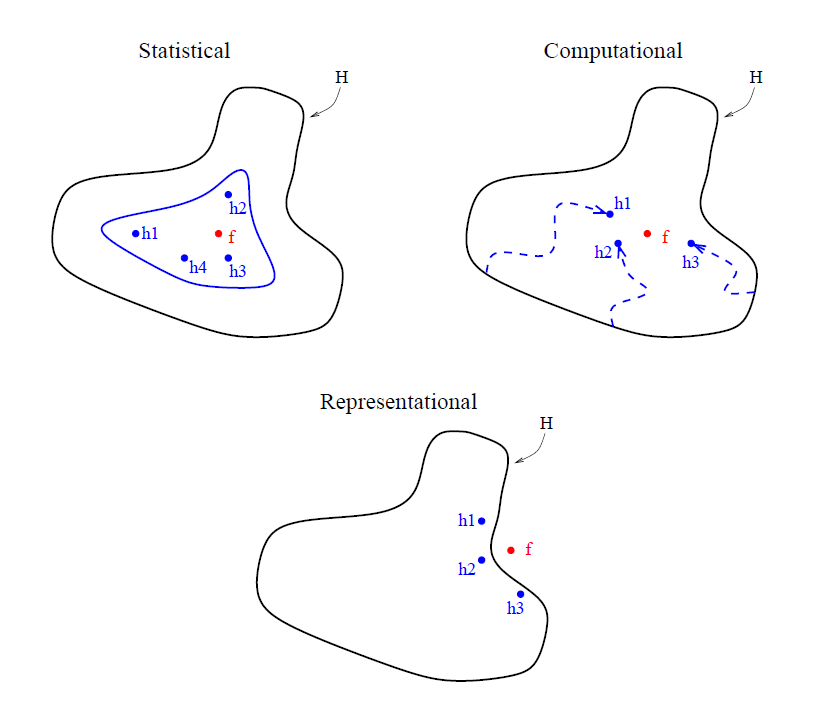
\includegraphics[scale = 0.4]{dietterich.png}
}

\frame{
  \frametitle{Implementation}
  The details of the ensemble implemented is describe here:

  \begin{itemize}
    \item {\textbf{Base learners:}}
      \begin{itemize}
        \item mean
        \item linear
        \item MARS
        \item exponential
        \item locally smooth linear
        \item logistic
        \item ARIMA
        \item naive
      \end{itemize}
      \item {\textbf{Combiner:}}
        non-trainable algebraic combiner - Weighted sum rule
        \begin{equation}
          u_j(x) = \sum_{i=1}^N w_i d_{n, j}(x) \nonumber
        \end{equation}
  \end{itemize}
  Where the weights depends on the fit on the available data.

}


\frame{
  \frametitle{}
  \includegraphics[scale = 0.4, page = 3]{productionEasy}
  %% Give several plots showing the different behaviour of the time
  %% series. (Both production and area harvested)
}


\frame{
  \frametitle{}
  \includegraphics[scale = 0.4, page = 3]{productionModerate}
  %% Give several plots showing the different behaviour of the time
  %% series. (Both production and area harvested)
}


\frame{
  \frametitle{}
  \includegraphics[scale = 0.4, page = 3]{productionDifficult2}
  %% Give several plots showing the different behaviour of the time
  %% series. (Both production and area harvested)
}


\frame{
  \frametitle{}
  \includegraphics[scale = 0.4, page = 3]{productionDifficult1}
  %% Give several plots showing the different behaviour of the time
  %% series. (Both production and area harvested)
}




\frame{
  \frametitle{}
  \includegraphics[scale = 0.4, page = 3]{productionHard1}
  %% Give several plots showing the different behaviour of the time
  %% series. (Both production and area harvested)
}


\frame{
  \frametitle{}
  \includegraphics[scale = 0.4, page = 3]{productionHard2}
  %% Give several plots showing the different behaviour of the time
  %% series. (Both production and area harvested)
}



\frame{
  \frametitle{}
  \includegraphics[scale = 0.4, page = 3]{productionImpossible}
  %% Give several plots showing the different behaviour of the time
  %% series. (Both production and area harvested)
}


\frame{
  \frametitle{Practical benefits of adopting the ensemble model}

  From the examples, we can see that we have an extremely flexible
  model with almost no possibility of over-fitting since none of the
  model are itself complex.

  \vfill

  We can continue to add in more models in which we consider appropriate.

  \vfill

  The reason it is called ensemble learning is becaues it is a model
  that can learn. If a production that has been growing linearly in
  the past but suddenly at an exponential rate, the model will learn
  and shift the weight of the linear model to model which are more
  flexible.
}


\frame{
  \frametitle{Explanatory variables?}
  Why we don't use other explanatory variables:

  \begin{itemize}
    \item Can contain as many missing value or more than our production
      domain.
    \item Too many of them, hard to choose from the set. A simple set
      would contain precipitation and temperature, should we also
      include number of sunny days? and their interactions? What about
      $\text{CO}_2$/phosphorus concentraction? Number of bee hives?
      Fertilizer, pesticide consumption?
    \item Difficult to maintain and integrate into the system.
  \end{itemize}
}


% \section{Balancing the Imputation}

% \frame{
%   \frametitle{}

%   After the initial imputation, we perform another step to balance the
%   individual imputation.

%   \vfill

%   This step is carried out to maintain the multivariate relationship
%   between the individual variables.

%   % This is done not only to satisfy the production equation
%   % (\ref{eq:pae}), but to maintain the multivariate relationship between
%   % the series.


%   \vfill

%   Maintaining the multivariate relasionthip is an important property
%   of imputation in particularly when they will be used for further
%   analysis.

% }

% \frame{
%   \frametitle{}

%   During this step, we not only adjust imputations performed in the
%   first step. But at the same time, we adjust values obtained from
%   sources other than official/semi-official.


%   \vfill

%   In the logged form of the identity, we can see that the relationship
%   is additive so we can simply maintain the relationship via a linear
%   regression. This is done by running a weighted spline regression.

%   \vfill

%   Official and semi-official sources will have a full weight of 1,
%   while other sources have currently been assigned a weight of 0.5.
%   % Explain the significance of the weighting and how we plan to
%   % estimate the weights from historical data.
% }

% % \frame{
% %   \frametitle{}
% %   In equation \ref{eq:lpae} we can see that the relationship is
% %   additive after taking the log. This also means we can tun a simple
% %   linear regression to maintain the relationship.
% %   To maintain the relationship, we regress the production on the yield
% %   and area harvested.
% %   However, we do not regress the production directly. Since we know
% %   the ratio change over time, we decompose the time series with cubic
% %   spline.
% % }



% \frame{
%   \frametitle{Further Improvements}
%   % (1) Improve the weighting through mining historical accuracy of
%   % different symbols.

% }



% \begin{frame}[allowframebreaks]
%   \frametitle{Reference}
%   \begin{thebibliography}{10}
%   \end{thebibliography}
% \end{frame}


\end{document}